%----------------------------------------------------------------------------------------
%	PACKAGES AND OTHER DOCUMENT CONFIGURATIONS
%----------------------------------------------------------------------------------------

\documentclass{article}

\usepackage{fancyhdr} % Required for custom headers
\usepackage{lastpage} % Required to determine the last page for the footer
\usepackage{extramarks} % Required for headers and footers
\usepackage[usenames,dvipsnames]{color} % Required for custom colors
\usepackage{graphicx} % Required to insert images
\usepackage{amsmath}% http://ctan.org/pkg/amsmath
\usepackage{listings} % Required for insertion of code
%\usepackage{couriernew} % Required for the courier font

\usepackage{enumerate} % Required for enumerating with letters

\usepackage{mathpazo}
\usepackage{avant}
\usepackage{inconsolata}

\usepackage{bm,upgreek}

\newcommand{\tr}{\text{tr}}
\newcommand{\pN}{\mathcal{N}}
\newcommand{\I}{\mathcal{I}}
\newcommand{\R}{\textsf{R} }
\newcommand{\1}{\mathbf{1}}
\newcommand{\0}{\mathbf{0}}
\newcommand{\x}{\mathbf{x}}
\newcommand{\tee}{\mathbf{t}}
\newcommand{\f}{\mathbf{f}}
\newcommand{\K}{\mathbf{K}}
\newcommand{\g}{\mathbf{g}}
\newcommand{\h}{\mathbf{h}}
\newcommand{\y}{\mathbf{y}}
\newcommand{\YY}{\mathbf{Y}}


% \newcommand{\1}{\bm{1}}
% \newcommand{\0}{\bm{0}}
% \newcommand{\x}{\bm{x}}
% \newcommand{\f}{\bm{f}}
% \newcommand{\y}{\bm{y}}

\newcommand{\iid}{\overset{\text{iid}}{\sim}}
\newcommand\independent{\protect\mathpalette{\protect\independenT}{\perp}}
\def\independenT#1#2{\mathrel{\rlap{$#1#2$}\mkern2mu{#1#2}}}

% Margins
\topmargin=-0.45in
\evensidemargin=0in
\oddsidemargin=0in
\textwidth=6.5in
\textheight=9.0in
\headsep=0.25in

\linespread{1.1} % Line spacing

% Set up the header and footer
\pagestyle{fancy}
\lhead{\hmwkAuthorName} % Top left header
\chead{\hmwkClass\ : \hmwkTitle} % Top center head
\rhead{} % Top right header
\lfoot{\lastxmark} % Bottom left footer
\cfoot{} % Bottom center footer
\rfoot{Page\ \thepage\ of\ \protect\pageref{LastPage}} % Bottom right footer
\renewcommand\headrulewidth{0.4pt} % Size of the header rule
\renewcommand\footrulewidth{0.4pt} % Size of the footer rule

\setlength\parindent{0pt} % Removes all indentation from paragraphs

%----------------------------------------------------------------------------------------
%	CODE INCLUSION CONFIGURATION
%----------------------------------------------------------------------------------------

\definecolor{MyDarkGreen}{rgb}{0.0,0.4,0.0} % This is the color used for comments
\lstloadlanguages{R} % Load R syntax for listings, for a list of other languages supported see: ftp://ftp.tex.ac.uk/tex-archive/macros/latex/contrib/listings/listings.pdf
\lstset{language=R, % Use R in this example
        frame=single, % Single frame around code
        basicstyle=\small\ttfamily, % Use small true type font
        keywordstyle=[1]\color{Blue}, % Perl functions bold and blue
        keywordstyle=[2]\color{Purple}, % Perl function arguments purple
        keywordstyle=[3]\color{Blue}\underbar, % Custom functions underlined and blue
        identifierstyle=, % Nothing special about identifiers                                         
        commentstyle=\usefont{T1}{pcr}{m}{sl}\color{MyDarkGreen}\small, % Comments small dark green courier font
        stringstyle=\color{Purple}, % Strings are purple
        showstringspaces=false, % Don't put marks in string spaces
        tabsize=4, % 5 spaces per tab
        %
        % Put standard Perl functions not included in the default language here
        morekeywords={rand},
        %
        % Put Perl function parameters here
        morekeywords=[2]{on, off, interp},
        %
        % Put user defined functions here
        morekeywords=[3]{test},
       	%
        morecomment=[l][\color{Blue}]{...}, % Line continuation (...) like blue comment
        numbers=left, % Line numbers on left
        firstnumber=1, % Line numbers start with line 1
        numberstyle=\tiny\color{Blue}, % Line numbers are blue and small
        stepnumber=5 % Line numbers go in steps of 5
}

% Creates a new command to include a perl script, the first parameter is the filename of the script (without .pl), the second parameter is the caption
\newcommand{\rscript}[2]{
\begin{itemize}
\item[]\lstinputlisting[caption=#2,label=#1]{#1.r}
\end{itemize}
}

%----------------------------------------------------------------------------------------
%	DOCUMENT STRUCTURE COMMANDS
%	Skip this unless you know what you're doing
%----------------------------------------------------------------------------------------

% Header and footer for when a page split occurs within a problem environment
\newcommand{\enterProblemHeader}[1]{
\nobreak\extramarks{#1}{#1 continued on next page\ldots}\nobreak
\nobreak\extramarks{#1 (continued)}{#1 continued on next page\ldots}\nobreak
}

% Header and footer for when a page split occurs between problem environments
\newcommand{\exitProblemHeader}[1]{
\nobreak\extramarks{#1 (continued)}{#1 continued on next page\ldots}\nobreak
\nobreak\extramarks{#1}{}\nobreak
}

\setcounter{secnumdepth}{0} % Removes default section numbers
\newcounter{homeworkProblemCounter} % Creates a counter to keep track of the number of problems

\newcommand{\homeworkProblemName}{}
\newenvironment{homeworkProblem}[1][Problem \arabic{homeworkProblemCounter}]{ % Makes a new environment called homeworkProblem which takes 1 argument (custom name) but the default is "Problem #"
\stepcounter{homeworkProblemCounter} % Increase counter for number of problems
\renewcommand{\homeworkProblemName}{#1} % Assign \homeworkProblemName the name of the problem
\section{\homeworkProblemName} % Make a section in the document with the custom problem count
\enterProblemHeader{\homeworkProblemName} % Header and footer within the environment
}{
\exitProblemHeader{\homeworkProblemName} % Header and footer after the environment
}

\newcommand{\problemAnswer}[1]{ % Defines the problem answer command with the content as the only argument
\noindent\framebox[\columnwidth][c]{\begin{minipage}{0.98\columnwidth}#1\end{minipage}} % Makes the box around the problem answer and puts the content inside
}

\newcommand{\homeworkSectionName}{}
\newenvironment{homeworkSection}[1]{ % New environment for sections within homework problems, takes 1 argument - the name of the section
\renewcommand{\homeworkSectionName}{#1} % Assign \homeworkSectionName to the name of the section from the environment argument
\subsection{\homeworkSectionName} % Make a subsection with the custom name of the subsection
\enterProblemHeader{\homeworkProblemName\ [\homeworkSectionName]} % Header and footer within the environment
}{
\enterProblemHeader{\homeworkProblemName} % Header and footer after the environment
}

%----------------------------------------------------------------------------------------
%	NAME AND CLASS SECTION
%----------------------------------------------------------------------------------------

\newcommand{\hmwkTitle}{Exercises 4 -- Hierarchical Models} % Assignment title
\newcommand{\hmwkDueDate}{\today} % Due date
\newcommand{\hmwkClass}{SDS\ 383D} % Course/class
\newcommand{\hmwkClassTime}{} % Class/lecture time
\newcommand{\hmwkClassInstructor}{Professor Scott} % Teacher/lecturer
\newcommand{\hmwkAuthorName}{Spencer Woody} % Your name

%----------------------------------------------------------------------------------------
%	TITLE PAGE
%----------------------------------------------------------------------------------------

\title{
\vspace{2in}
\textmd{\textbf{\hmwkClass:\ \hmwkTitle}}\\
\normalsize\vspace{0.1in}\small{\hmwkDueDate}\\
\vspace{0.1in}\large{\textit{\hmwkClassInstructor\ }}
\vspace{3in}
}

\author{\textbf{\hmwkAuthorName}}
\date{} % Insert date here if you want it to appear below your name

%----------------------------------------------------------------------------------------

\begin{document}

\maketitle

\newpage

%----------------------------------------------------------------------------------------
%	PROBLEM 1
%----------------------------------------------------------------------------------------

\begin{homeworkProblem}

\large
\textbf{Math Tests}
\normalsize

We have a model where $y_{ij}$ is the test score of the $j$th student in school $i$, with indices $i = 1, 2, \ldots, I$ and $j = 1, 2, \ldots, N_i,$ so $N_i$ is the sample size for school $i$ and there are $N = \sum_{i=1}^I$ total test scores. Let $\lambda = 1/\sigma^2$ and $\gamma = 1/\tau^2$ be the precision parameters. Further, let $y_i = [y_{i1}, y_{i2}, \ldots, y_{iN_i}]^T$ and $y = [y_1^T, y_2^T, \ldots, y_I^T]^T$ and $\theta = [\theta_1, \theta_2, \ldots, \theta_I]^T.$ As we can see in Figure \ref{fig:mathscatter}, schools with smaller sample sizes tend to have more extreme average test scores.

\begin{figure}[htp!]
	\centering
		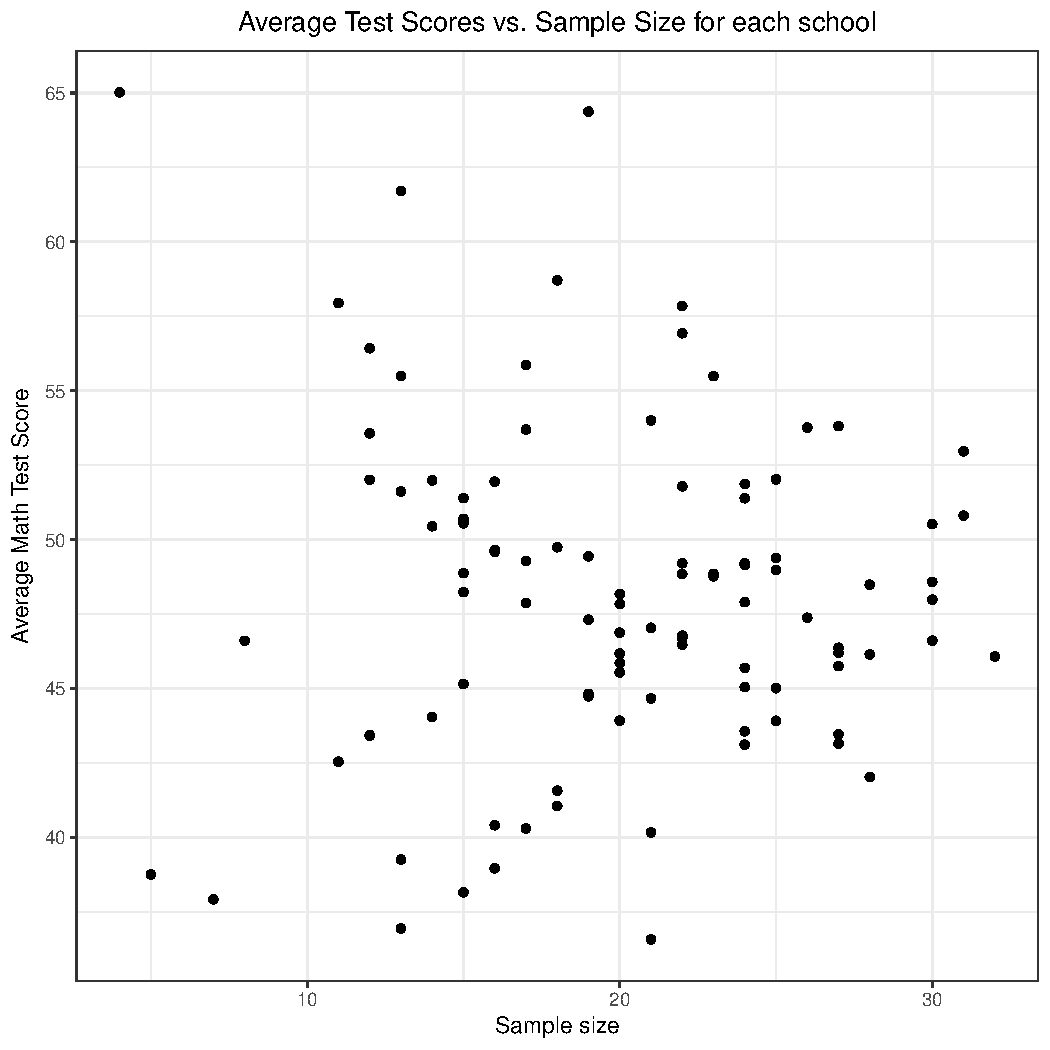
\includegraphics[scale=0.5]{Math/img/scatter.pdf}
	\caption{Scatter plot of sample size and average test scores}
	\label{fig:mathscatter}
\end{figure}

 The hierarchical model for these data is 
%
%
%
\begin{align*}
	(y_{ij} | \theta_i, \lambda) &\sim \pN\left(\theta_i, \lambda^{-1}\right) \\
	(\theta_i | \mu, \lambda, \gamma) &\sim \pN\left(\mu, (\lambda \gamma)^{-1}\right).
\end{align*}
%
%
We set the priors 
%
%
%
\begin{align*}
	\pi(\mu) &\propto 1,\; -\infty < \mu < \infty \\
	\pi(\lambda) &\propto \lambda^{-1},\; \lambda > 0 \\
	\pi(\gamma) &\propto 1,\; \gamma > 0,
\end{align*}
%
%
%
that is to say, \ldots. In order to implement the Gibbs sampler, we need the posterior full conditionals for each $\theta_i$, $\mu$, $\lambda$, and $\gamma$.
%
%
%
\begin{itemize}
	\item For each $\theta_i,$ 
	%
	%
	%
	\begin{align*}
		f(\theta_i | y_i, \mu, \lambda, \gamma) &\propto f(y_i | \theta_i, \lambda) \cdot f(\theta_i | \mu, \lambda, \gamma) \\
		&\sim \pN \left( (N_i\lambda + \lambda \gamma)^{-1} \cdot (N_i \lambda \bar{y}_i + \lambda \gamma \mu), (N_i\lambda + \lambda \gamma)^{-1} \right),
	\end{align*}
	%
	%
	%
	which we know from the normal-normal conjugacy derived in Exercises 1.
	%
	%
	%
	\item For $\mu$,
	%
	%
	%
	\begin{align*}
		\pi(\mu | y, \theta, \lambda, \gamma) &\propto f(\theta | \lambda, \gamma, \mu) \cdot \pi(\mu) \\
		&\propto \left( \prod_{i = 1}^I \exp \left[ -\frac{1}{2} \lambda \gamma (\theta_i - \mu)^2 \right] \right) \cdot 1 \\
		&= \exp \left[ -\frac{1}{2} \lambda \gamma \sum_{i=1}^I (\theta_i - \mu)^2 \right] \\
		&= \exp \left[ -\frac{1}{2} \lambda \gamma \sum_{i=1}^I \left( \theta_i^2 - 2\theta_i \mu + \mu^2 \right) \right] \\
		&\propto \exp \left[ -\frac{1}{2} \lambda \gamma \left( I\mu^2 - 2I\bar{\theta} \mu \right) \right] \\
		&\sim \pN \left( \bar{\theta}, (I\lambda \gamma)^{-1} \right).
	\end{align*}
	%
	%
	%
	\item For $\lambda$,
	%
	%
	%
	\begin{align*}
		\pi(\lambda | y, \mu, \gamma, \theta) &\propto f(y | \lambda, \theta) \cdot f(\theta | \lambda, \gamma, \mu) \cdot \pi(\lambda) \\
		%
		&\propto \left( \prod_{i = 1}^I \prod_{j=1}^{N_i} \lambda^{1/2} \exp \left[ -\frac{1}{2} (y_{ij} - \theta_i)^2 \right] \right) \cdot \left( \prod_{i=1}^I \lambda^{1/2} \exp \left[ -\frac{1}{2} \lambda \gamma (\theta_i - \mu)^2 \right] \right) \cdot \lambda^{-1} \\
		%
		&= \lambda^{(N+I)/2 - 1} \exp \left[ -\frac{1}{2} \left( \sum_{i=1}^I \sum_{j=1}^{N_i} (y_{ij} - \theta_i)^2 + \gamma \sum_{i=1}^I (\theta_i - \mu)^2 \right) \lambda \right] \\
		%
		&\sim \text{Gamma} \left( \frac{N+I}{2}, \frac{1}{2} \left[ \sum_{i=1}^I \sum_{j=1}^{N_i} (y_{ij} - \theta_i)^2 + \gamma \sum_{i=1}^I (\theta_i - \mu)^2 \right] \right).
	\end{align*}
	
	%
	%
	%
	\item For $\gamma$,
	%
	%
	%
	\begin{align*}
		\pi(\gamma | y, \mu, \lambda, \theta) &\propto f(\theta | \lambda, \gamma, \mu) \cdot \pi(\gamma) \\
		%
		&\propto \left( \prod_{i+1}^I \gamma^{1/2} \exp \left[ - \frac{1}{2} \lambda \gamma (\theta_i - \mu)^2 \right] \right) \cdot 1 \\
		%
		&= \gamma^{I/2} \exp\left[- \frac{1}{2} \lambda \sum_{i=1}^I (\theta_i - \mu)^2 \cdot \gamma \right] \\
		&\sim \text{Gamma}\left( \frac{I}{2} + 1, \frac{1}{2}\lambda \sum_{i=1}^I (\theta_i - \mu)^2  \right).
	\end{align*}
	%
	%
	%
\end{itemize}

\begin{table}[htp!]
\centering
\caption{95\% posterior credible intervals}
\begin{tabular}{r|rrr}
  \hline
 & 2.5\% & 50\% & 97.5\% \\ 
  \hline
$\mu$ & 47.03 & 48.10 & 49.18 \\ 
  $\lambda$ & 0.0111 & 0.0118 & 0.0126 \\ 
  $\gamma$ & 2.43 & 3.49 & 5.03 \\ 
   \hline
\end{tabular}
\end{table}

Given the posterior mean $\hat{\theta}_i$ as an estimate of $\theta_i,$ define the shrinkage coefficient $$\kappa_i = \frac{\bar{y}_i - \hat{\theta}_i}{\bar{y}_i},$$ which is a measure incomplete pooling. Figure \ref{fig:mathkappa} shows the absolute shrinkage coefficient for each school as a function of sample size. As sample size increases, the shrinkage decreases because we are gaining precision in estimating the school-level mean $\theta_i.$

\begin{figure}[htp!]
	\centering
		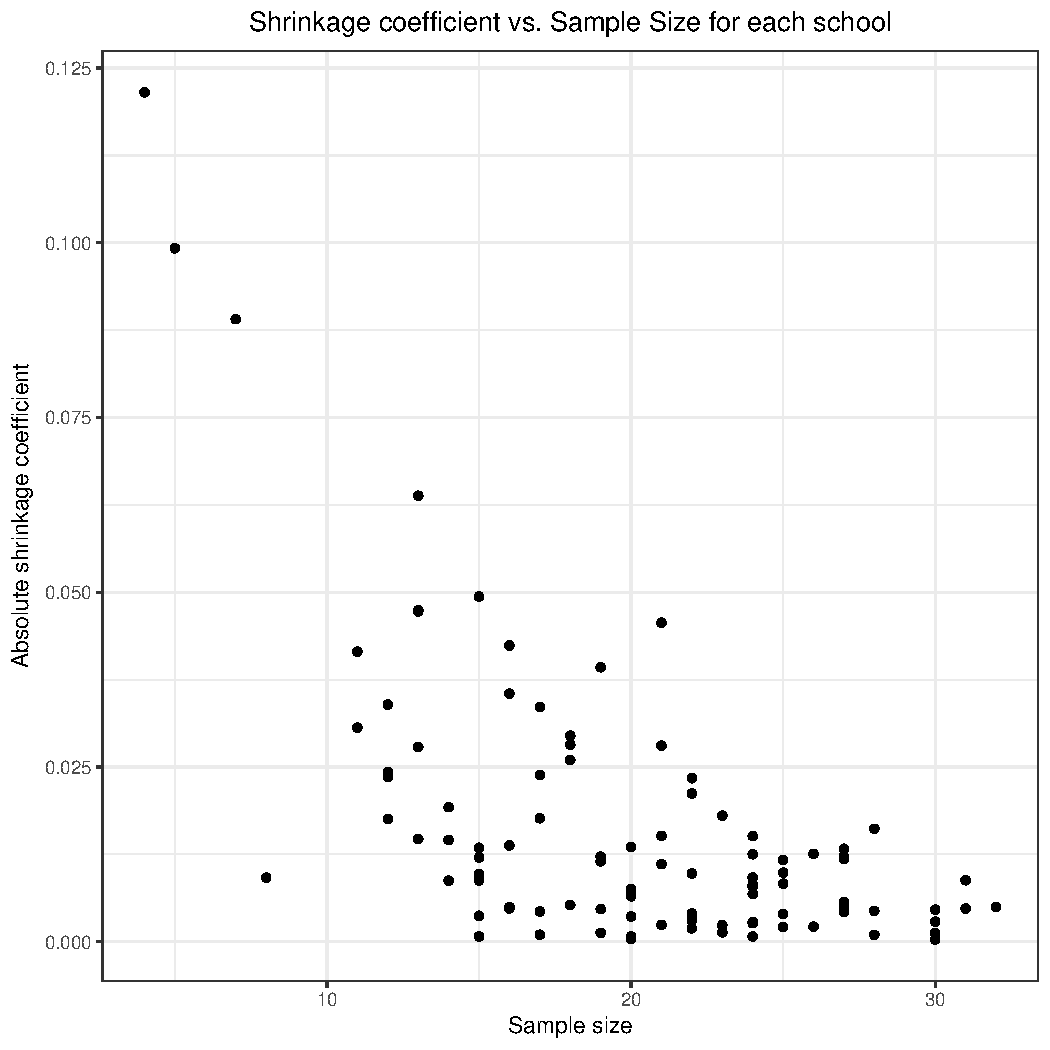
\includegraphics[scale=0.65]{Math/img/kappa.pdf}
	\caption{Absolute shrinkage coefficient as a function of sample size}
	\label{fig:mathkappa}
\end{figure}


\end{homeworkProblem}

%----------------------------------------------------------------------------------------
%	PROBLEM 2
%----------------------------------------------------------------------------------------

\pagebreak

\begin{homeworkProblem}

\large
\textbf{Price elasticity of demand}
\normalsize

Here we model the demand curve for cheese, which is given by $$ Q =  \alpha P ^\beta,$$ where $Q$ is the quantity of cheese demanded, $P$ is price, $\beta$ is a parameter for the \emph{price elasticity of demand} and $\alpha$ is a (rather unremarkable) scaling parameter. Note that if we take a logarithmic transform of the equation in our demand model, we obtain the linear replationship $$ \log Q = \log \alpha + \beta \log P. $$ Figure \ref{fig:cheesescatter} shows all the data with a fitted OLS line, and Figure \ref{fig:OLSfacetplot} shows the data on a store-by-store level with the same OLS line from all data on each panel. The fact that the OLS line performs poorly on any given individual store's data suggests that a hierarchical approach would be beneficial. The hierarchical linear model for the quantity of cheese sold for the $t$th observation at store $i$ is
%
\begin{align*}
	y_{it} &= \alpha_i + \beta_i x_{it} + \gamma_i z_{it} + \theta_i z_{it} x_{it} + \epsilon_{it},
\end{align*} 
% 
where $x_{it}$ is the log-price of cheese and $z_{it}$ is an indicator variable taking on a value of 1 when the display is shown, and 0 otherwise.
%
\begin{figure}[htp!]
	\centering
		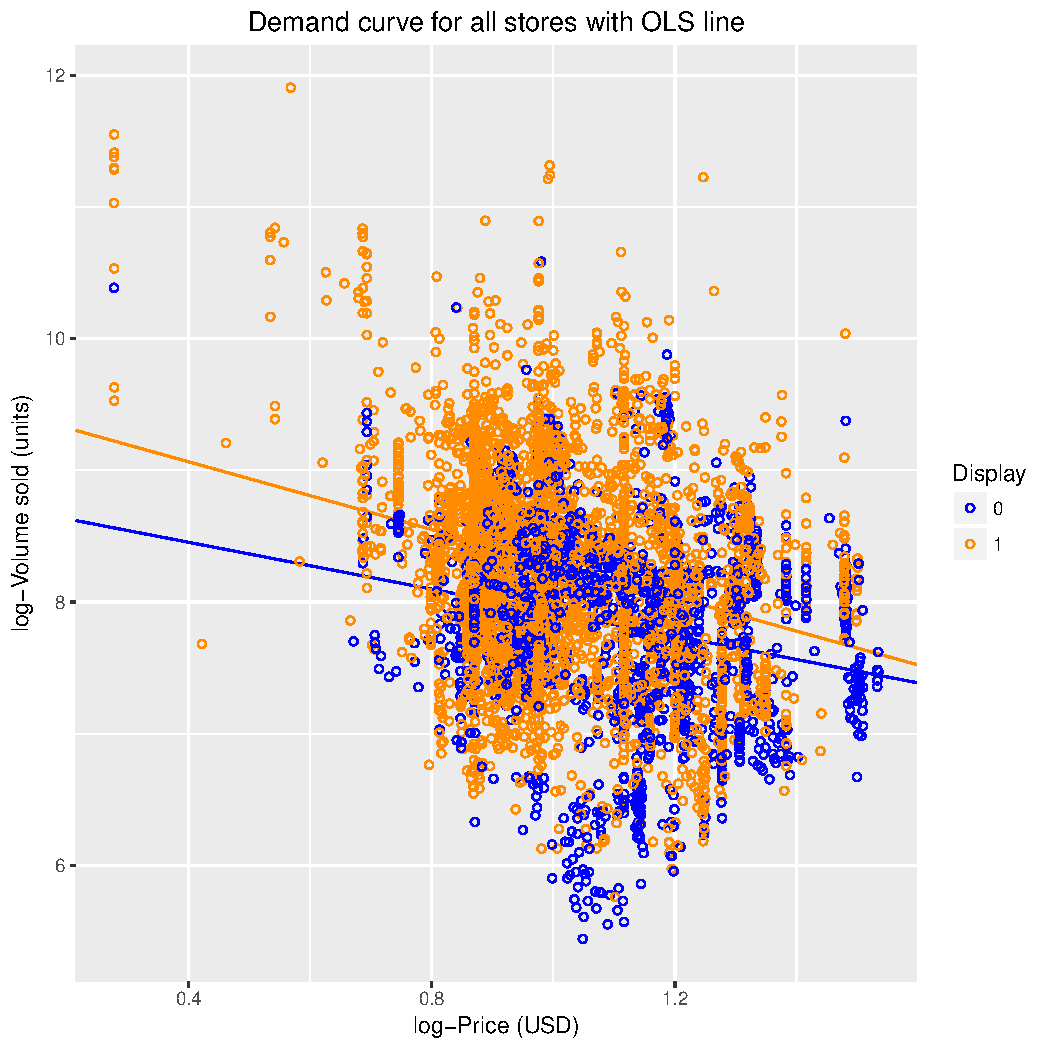
\includegraphics[scale=0.5]{Cheese/img/OLSplot.pdf}
	\caption{Scatterplot for data from all stores with OLS line}
	\label{fig:cheesescatter}
\end{figure}

\begin{figure}[htp!]
	\centering
		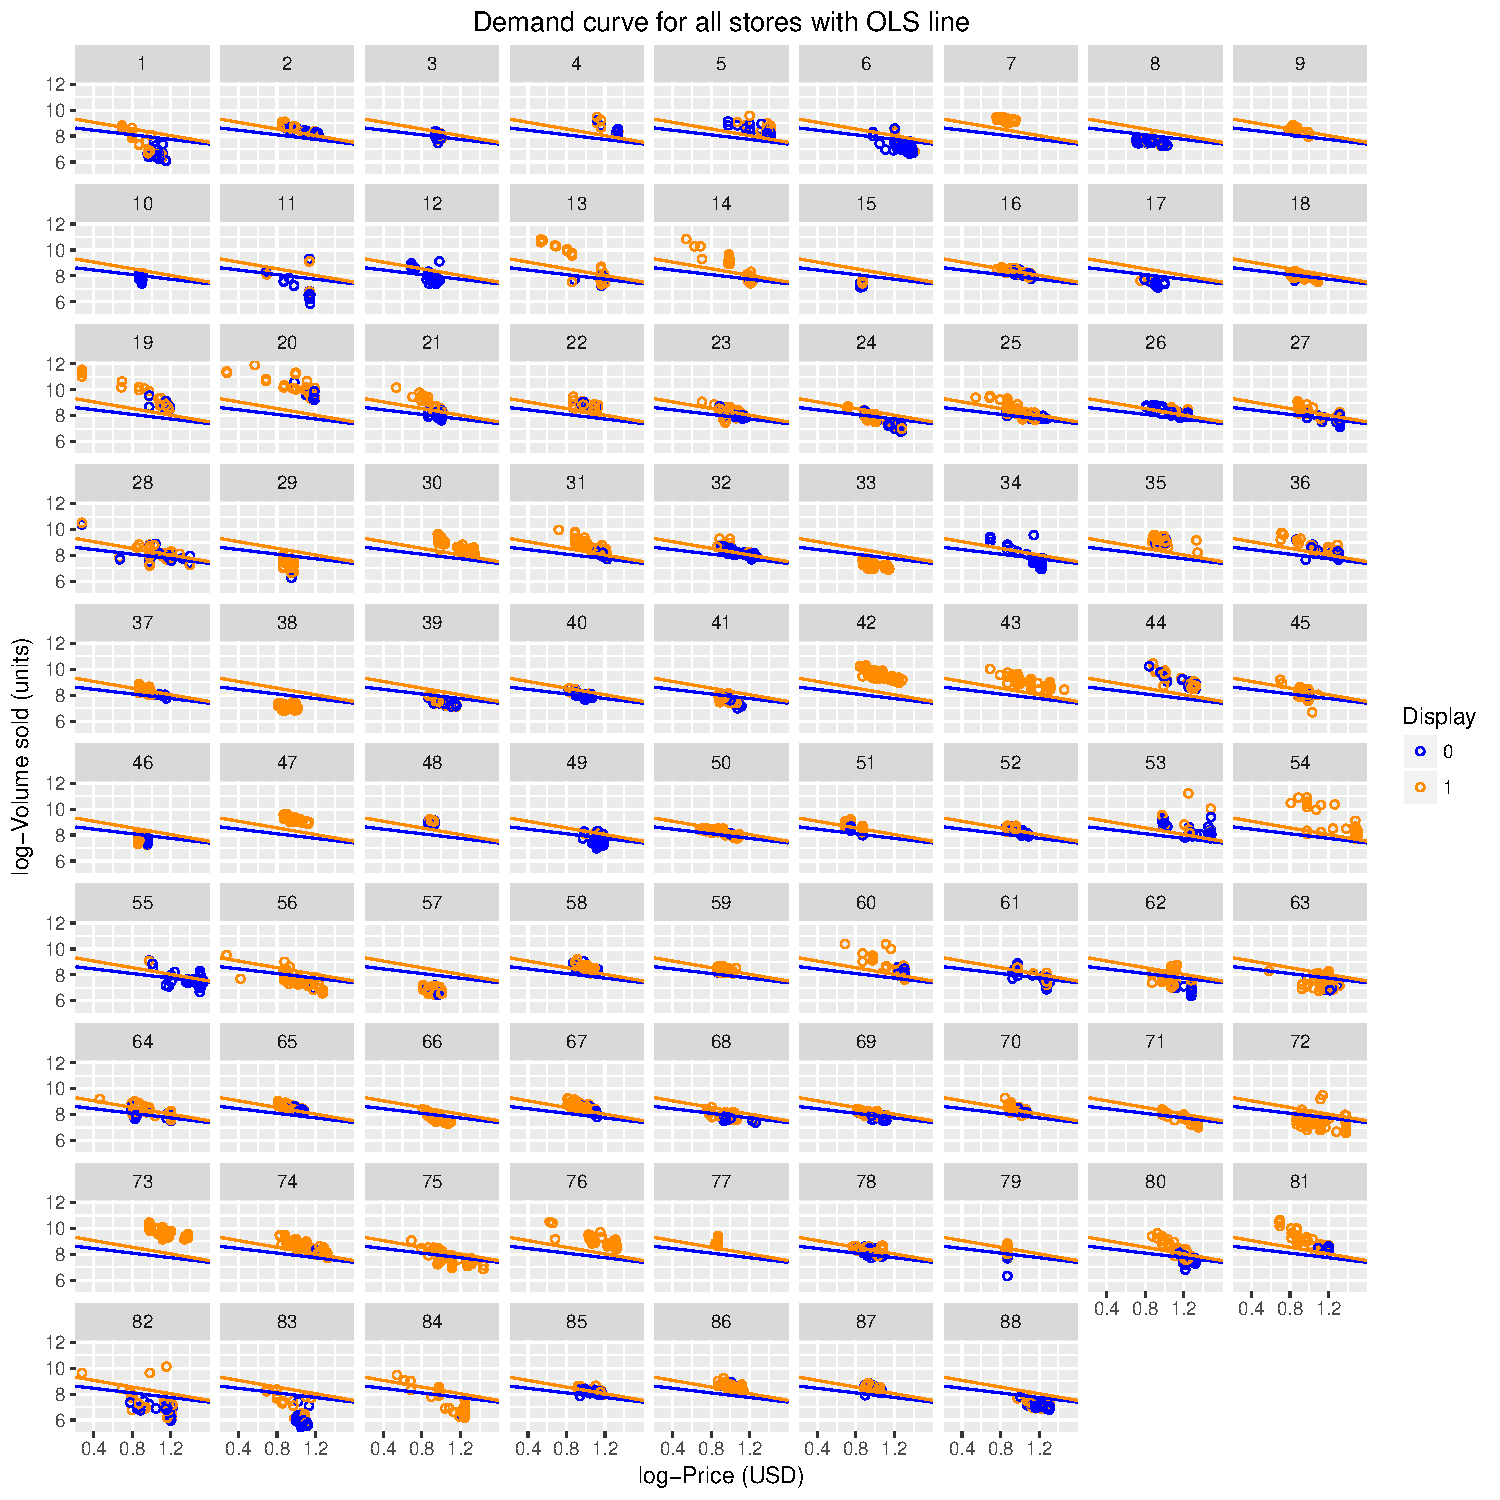
\includegraphics[scale=0.7]{Cheese/img/OLSfacetplot.pdf}
	\caption{Scatterplot for data from all stores with OLS line}
	\label{fig:OLSfacetplot}
\end{figure}
%
Using freqentist REML to build this model we obtain these results, 
%
\begin{figure}[htp!]
	\centering
		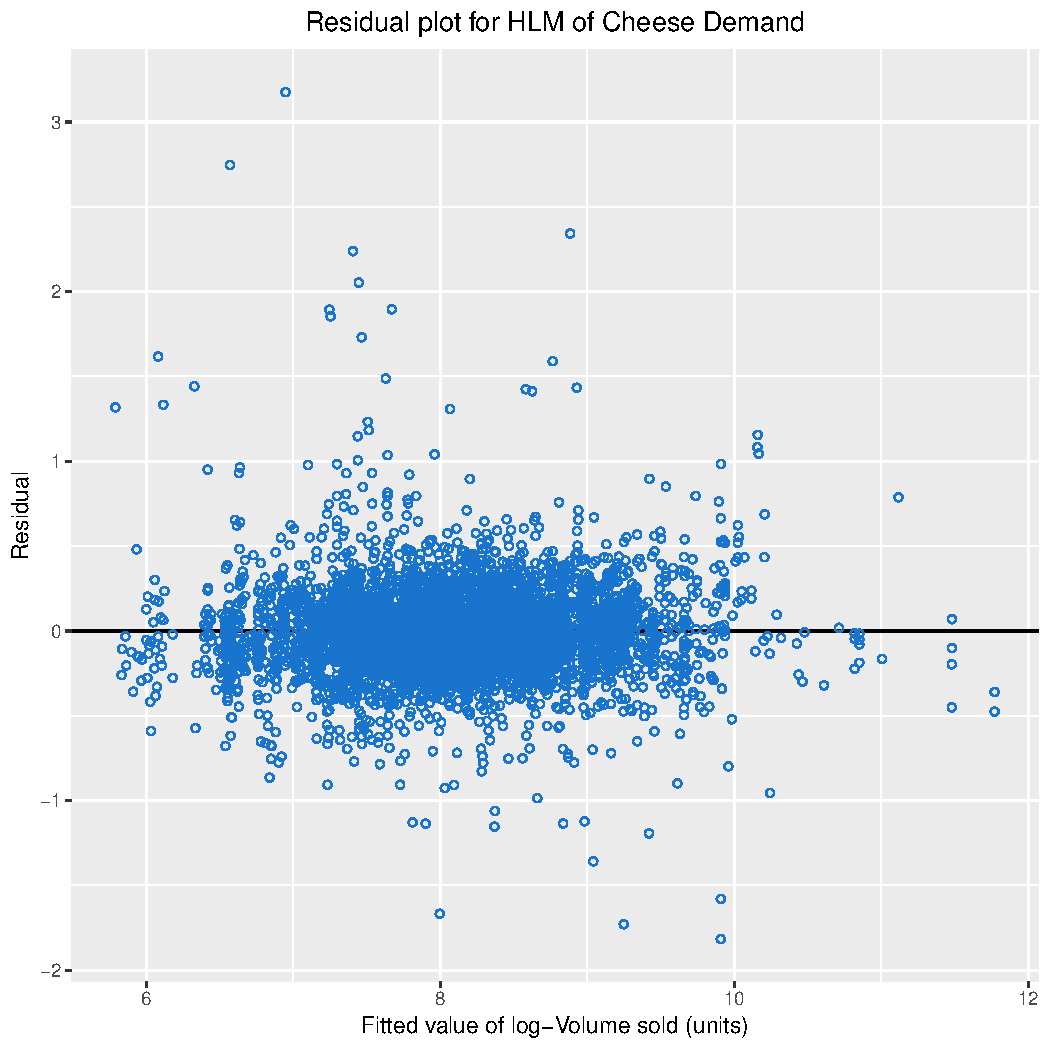
\includegraphics[scale=0.5]{Cheese/img/cheeseresid1.pdf}
	\caption{Residual plot using HLM and REML method}
	\label{fig:cheeseresid1}
\end{figure}

\pagebreak

\emph{Full Bayesian}

\textbf{Model specification} 

Here we specify a general Bayesian hierarchical linear model. Let $y_i$ be a $n_i$-length vector representing the the responses of group $i.$ There are $N = \sum_{i}^I n_i$ total responses. $X_i$ is the $n_i \times p$ design matrix for the observations in group $i$, and $Z_i$ is a $n_i \times q,$ $q \leq p$ matrix whose columns are a subset of the columns of $X_i$, and this represents the subject-level effects, sometimes called ``random effects.''. Then the responses $y_i$ are distributed as: 
%
\begin{align*}
	y_{i} | \beta, b_i, \lambda &\sim \pN_{n_i}(X_i \beta + Z_ib_i, \lambda^{-1}\I_{n_i}) \\
	b_i | D &\iid \pN_{q} (0, D)
\end{align*}
%
%
%
Note that the responses $y_{it}$ for subject $i$ are therefore assumed to iid, and also note two results of this model, 
%
%
\begin{align*}
	E(y_{i} | b_i) &= X_i \beta + Z_ib_i \\
	E(y_{i}) &= E(E(y_{i} | b_i)) = X_i \beta,
\end{align*}
%
%
or in other words, 
%
%
The priors are
%
%
\begin{align*}
	\pi(\lambda) &\propto \lambda^{-1} \\
	\pi(\beta) &\propto 1 \\
	\pi(D) &\sim \text{IW}(\nu, \Psi).
\end{align*}
% 
%
To implement a Gibbs sampler, we need the full conditional posterior distributions for $b_i$, $\lambda$, $\beta$, and $D$.
%
%
\begin{itemize}
	\item %
	For each $b_i$, first define $v_i := y_i - X_i \beta,$
	%
	%
	\begin{align*}
		p(b_i | y_i, \lambda, \beta, D) &\propto p(y_i | \beta, b_i, \lambda) p(b_i | D) \\ 
		%
		&\propto \exp \left[ -\frac{1}{2} \lambda \left( y_i - X_i \beta - Z_i b_i \right)^T \left( y_i - X_i \beta - Z_i b_i \right)  \right] \cdot \exp \left[ -\frac{1}{2} b_i^T D^{-1} b_i \right] \\
		%
		&= \exp \left[ -\frac{1}{2} \lambda \left( Z_i b_i - v_i \right)^T \left( Z_i b_i - v_i \right)  \right] \cdot \exp \left[ -\frac{1}{2} b_i^T D^{-1} b_i \right] \\
		%
		&\propto \exp\left[ -\frac{1}{2} b_i^T \left( \lambda Z_i^TZ_i + D^{-1} \right) b_i - 2b_i^T\lambda Z_i^T v_i \right] \\
		%
		&\propto \exp \left[ -\frac{1}{2} \left( b_i - \left[ \lambda Z_i^T Z_i + D^{-1} \right]^{-1} \lambda Z_i^T v_i \right)^T \left( \lambda Z_i^T Z_i + D^{-1}  \right) \left( b_i - \left[ \lambda Z_i^T Z_i + D^{-1} \right]^{-1} \lambda Z_i^T v_i \right) \right] \\
		% 
		&\sim \pN \left( \left[ \lambda Z_i^T Z_i + D^{-1} \right]^{-1} \lambda Z_i^T v_i, \left[ \lambda Z_i^T Z_i + D^{-1} \right]^{-1} \right). \\
		%
		&\sim \pN \left( \left[ \lambda Z_i^T Z_i + D^{-1} \right]^{-1} \lambda Z_i^T (y_i - X_i \beta), \left[ \lambda Z_i^T Z_i + D^{-1} \right]^{-1} \right).
	\end{align*}
	%
	%
	\item 
	For $\lambda,$
	%
	%
	\begin{align*}
		\pi(\lambda| y, \beta, b) &\propto p(y | \lambda, \beta, \b) \cdot \pi(\lambda) \\
		&= \left( \prod_{i=1}^I \lambda^{n_i/2} \exp \left[ -\frac{1}{2} \lambda (y_i - X_i\beta - Z_ib_i)^T (y_i - X_i\beta - Z_ib_i) \right] \right) \cdot \lambda^{-1} \\
		%
		&\sim \text{Gamma}\left( \frac{N}{2}, \frac{1}{2} \sum_{i=1}^I \| y_i - X_i\beta - Z_ib_i \|^2_2 \right)
	\end{align*}
	%
	%
	\item %
	For $\beta,$ define $w_i := y_i - Z_ib_i. $
	%
	%
	\begin{align*}
		\pi(\beta| y, \lambda, b) &\propto p(y | \lambda, \beta, \b) \cdot \pi(\beta) \\
		%
		&\propto \left( \prod_{i=1}^I \exp \left[ -\frac{1}{2} \lambda (y_i - X_i\beta - Z_ib_i)^T (y_i - X_i\beta - Z_ib_i) \right] \right) \cdot 1 \\
		%
		&= \prod_{i=1}^I \exp \left[ -\frac{1}{2} \lambda (X_i\beta - w_i)^T (X_i\beta - w_i) \right] \\
		%
		&\propto \prod_{i=1}^I \exp \left[ -\frac{1}{2} \lambda \left( \beta^T X_i^T X_i \beta - 2\beta^TX_i^T w_i \right) \right] \\
		%
		&= \exp\left( -\frac{1}{2} \lambda \left[ \beta^T \left( \sum_{i=1}^I X_i^T X_i \right)\beta - 2\beta^T \sum_{i=1}^I X_i^T w_i \right] \right) \\
		%
		&=  \exp\left( -\frac{1}{2} \lambda \left[ \beta^T \left( \sum_{i=1}^I X_i^T X_i \right)\beta - 2\beta^T \sum_{i=1}^I X_i^T (y_i - Z_ib_i) \right] \right) \\ 
		%
		&\sim \pN \left( \left[ \sum_{i=1}^I X_i^T X_i \right]^{-1} \sum_{i=1}^I X_i^T (y_i - Z_ib_i), \left[ \lambda \sum_{i=1}^I X_i^T X_i \right]^{-1} \right).
	\end{align*}
	%
	%
	\item
	For $D,$
	%
	%
	\begin{align*}
		\pi(D | b) &\propto p(b | D) \cdot \pi(D) \\
		&\propto \left( \prod_{i=1}^I [\det(D)]^{-1/2} \exp \left[ -\frac{1}{2} b_i^T D^{-1} b_i \right] \right) \cdot [\det(D)]^{- \frac{\nu + q + 1}{2}} \exp\left[ -\frac{1}{2} \tr(\Psi D^{-1}) \right] \\
		&\sim \text{IW}\left( I + \nu, \Psi + \sum_{i=1}^I b_ib_i^T \right)
	\end{align*}
\end{itemize}

The most computationally intensive part of this Gibbs sampler scheme is sampling each $b_i,$ and I chose to do this by exploiting a block-diagonal matrix of each $Z_i$ and drawing each $b_i$ simultaneously as a long vector called $b$. For this application specifically, the $X_i$ and $Z_i$ are identical, with a column of 1's for the intercept, a column of log-prices, a column of indicator variables for display, and a column of interaction terms for log-price and display. We run 6000 iterations of the Gibbs sampler with the first 1000 draws discared as burn-in. The \texttt{mix} folder within the \texttt{img} folder shows traceplots of $\lambda$, each component in $\beta$, and four randomly selected columns of posterior draws of $b$, which all show a good degree of mixing. Histograms for $lambda$ and each component of $\beta$ are shown below. Figure \ref{fig:CIgrid} shows a grid of plots, each of which has 95\% credible intervals of all the subject-level effects on a given covariate terms, arranged in increasing order by posterior median. Note that on the $x$-axis is different for each plot in order to have each one ordered by posterior median. 

\begin{figure}[htp!]
	\centering
		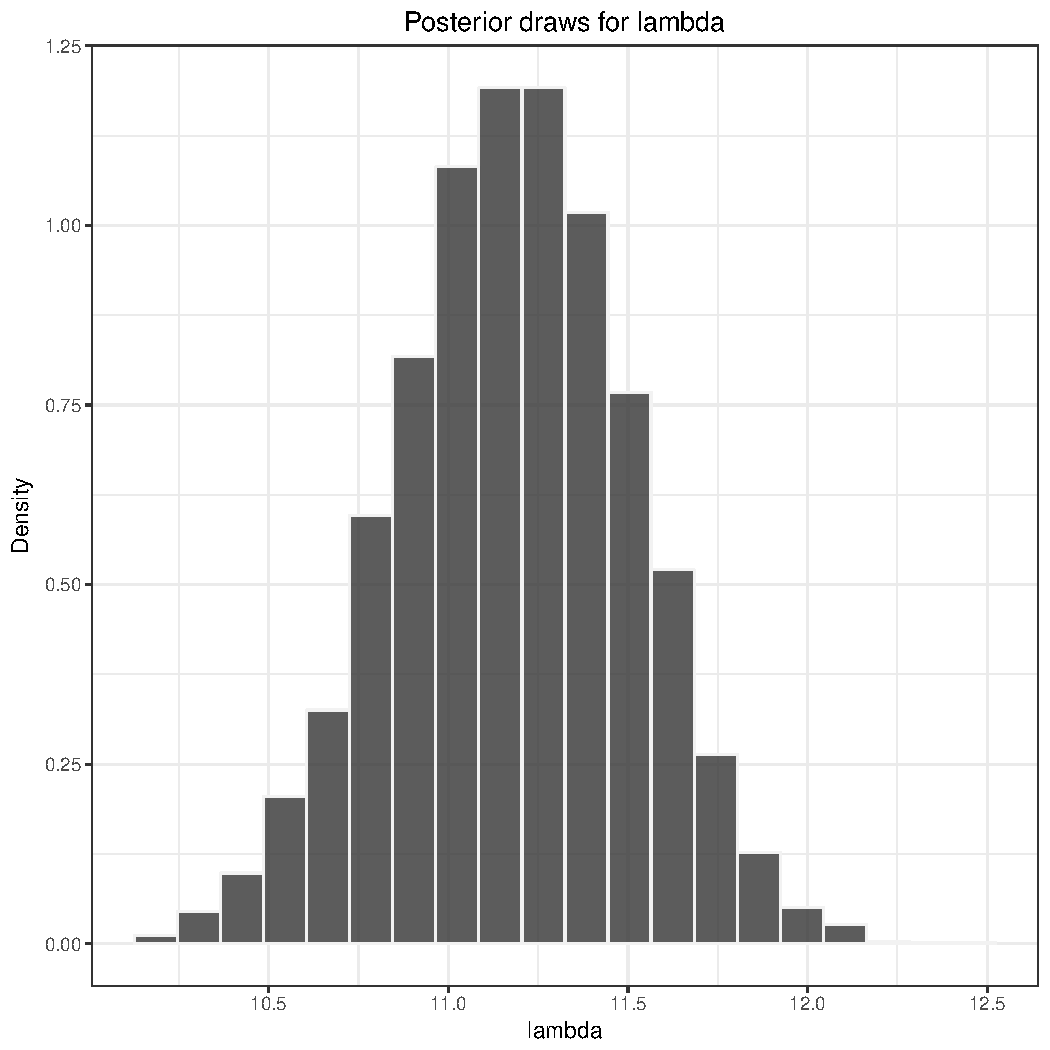
\includegraphics[scale=0.4]{Cheese/img/hist/lambdahist.pdf}
	\caption{Histogram of posterior draws of $\lambda$}
\end{figure}

\begin{figure}[htp!]
	\centering
		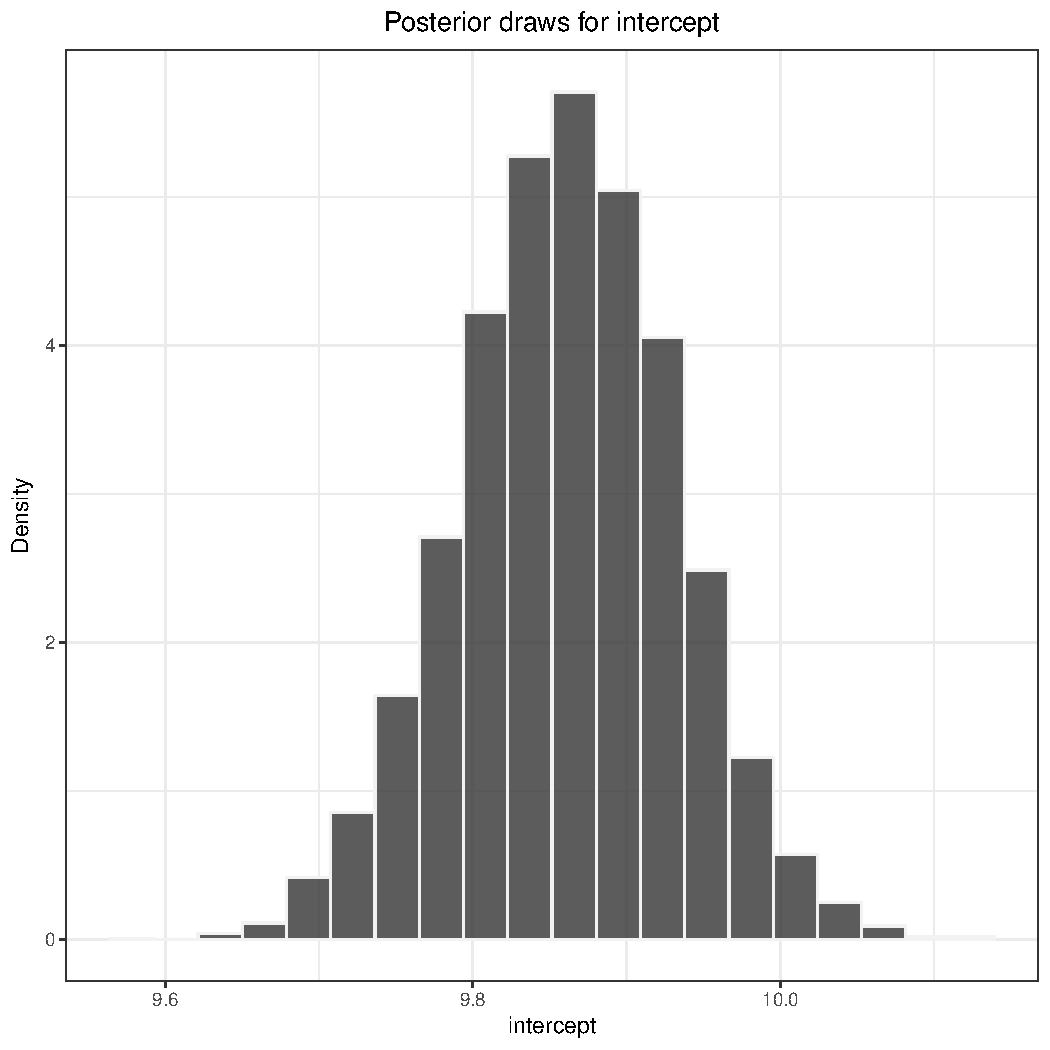
\includegraphics[scale=0.4]{Cheese/img/hist/inthist.pdf}
		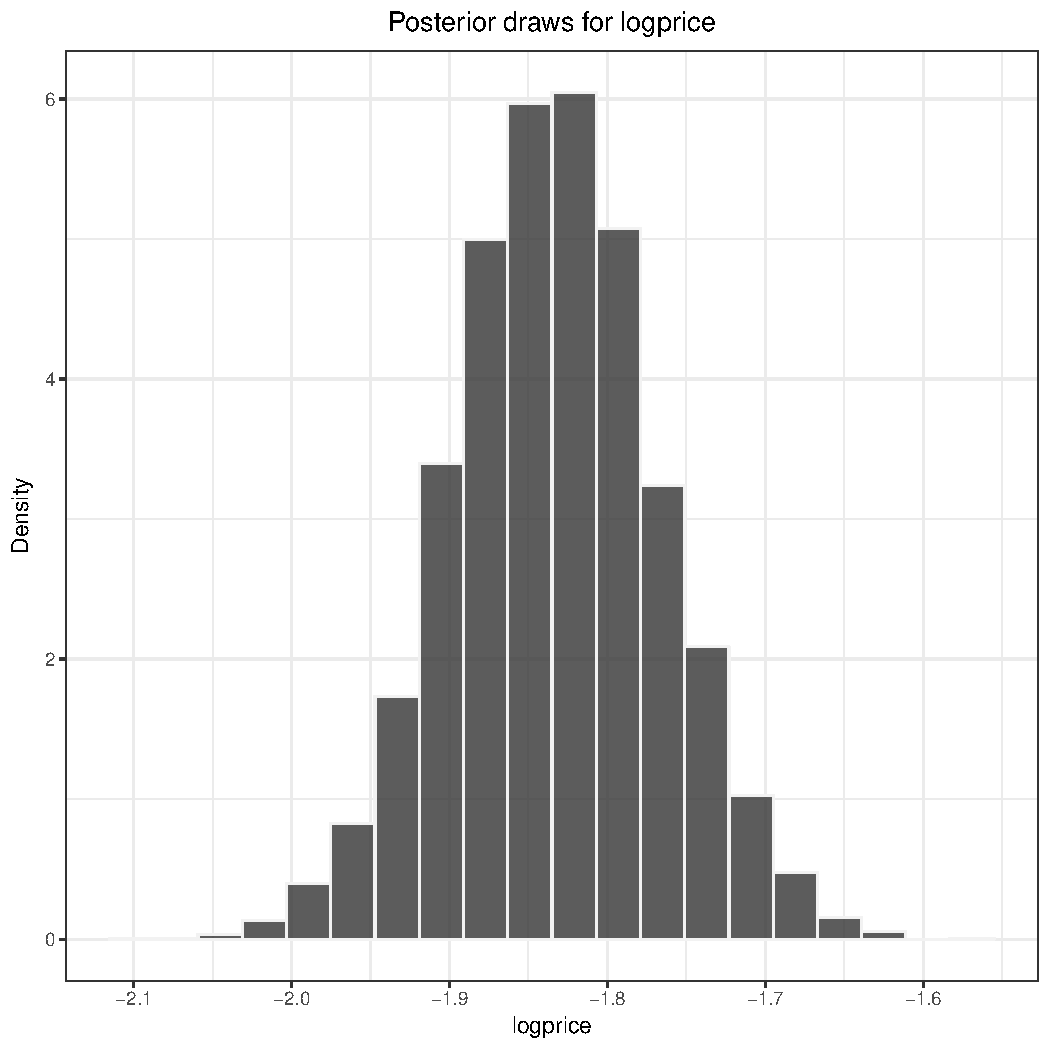
\includegraphics[scale=0.4]{Cheese/img/hist/logpricehist.pdf} \\
		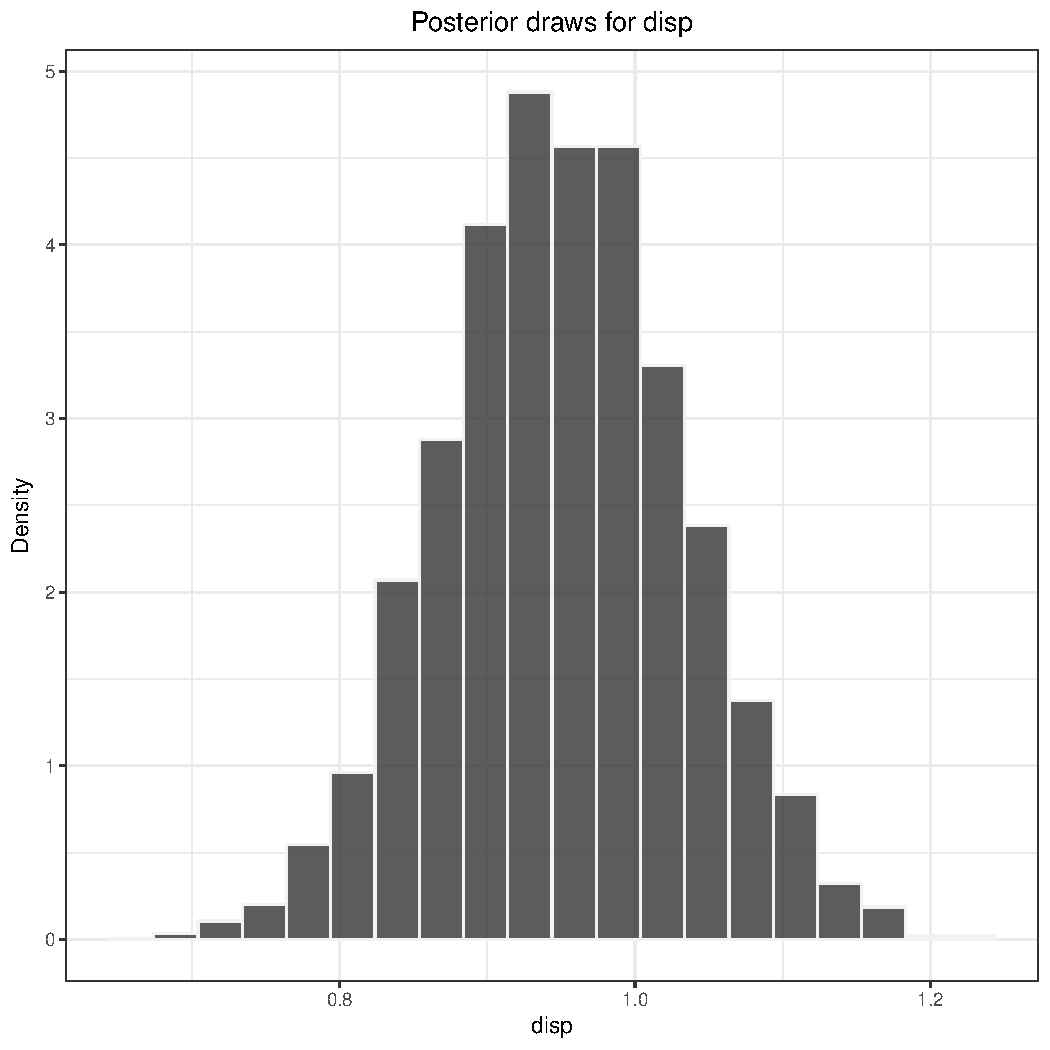
\includegraphics[scale=0.4]{Cheese/img/hist/disphist.pdf}
		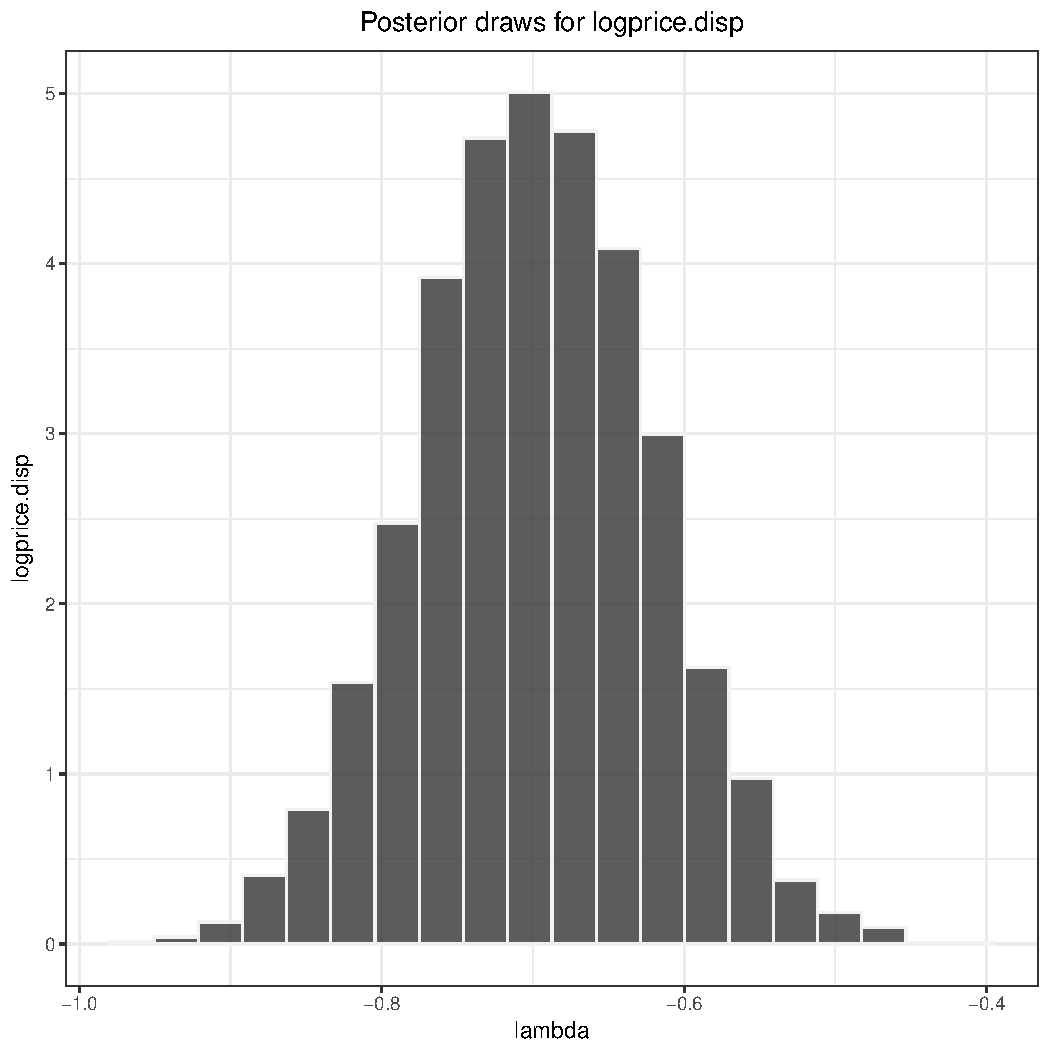
\includegraphics[scale=0.4]{Cheese/img/hist/logprice_disphist.pdf}
	\caption{Histogram of posterior draws of each term in $\beta$}
\end{figure}

\begin{figure}[htp!]
	\centering
		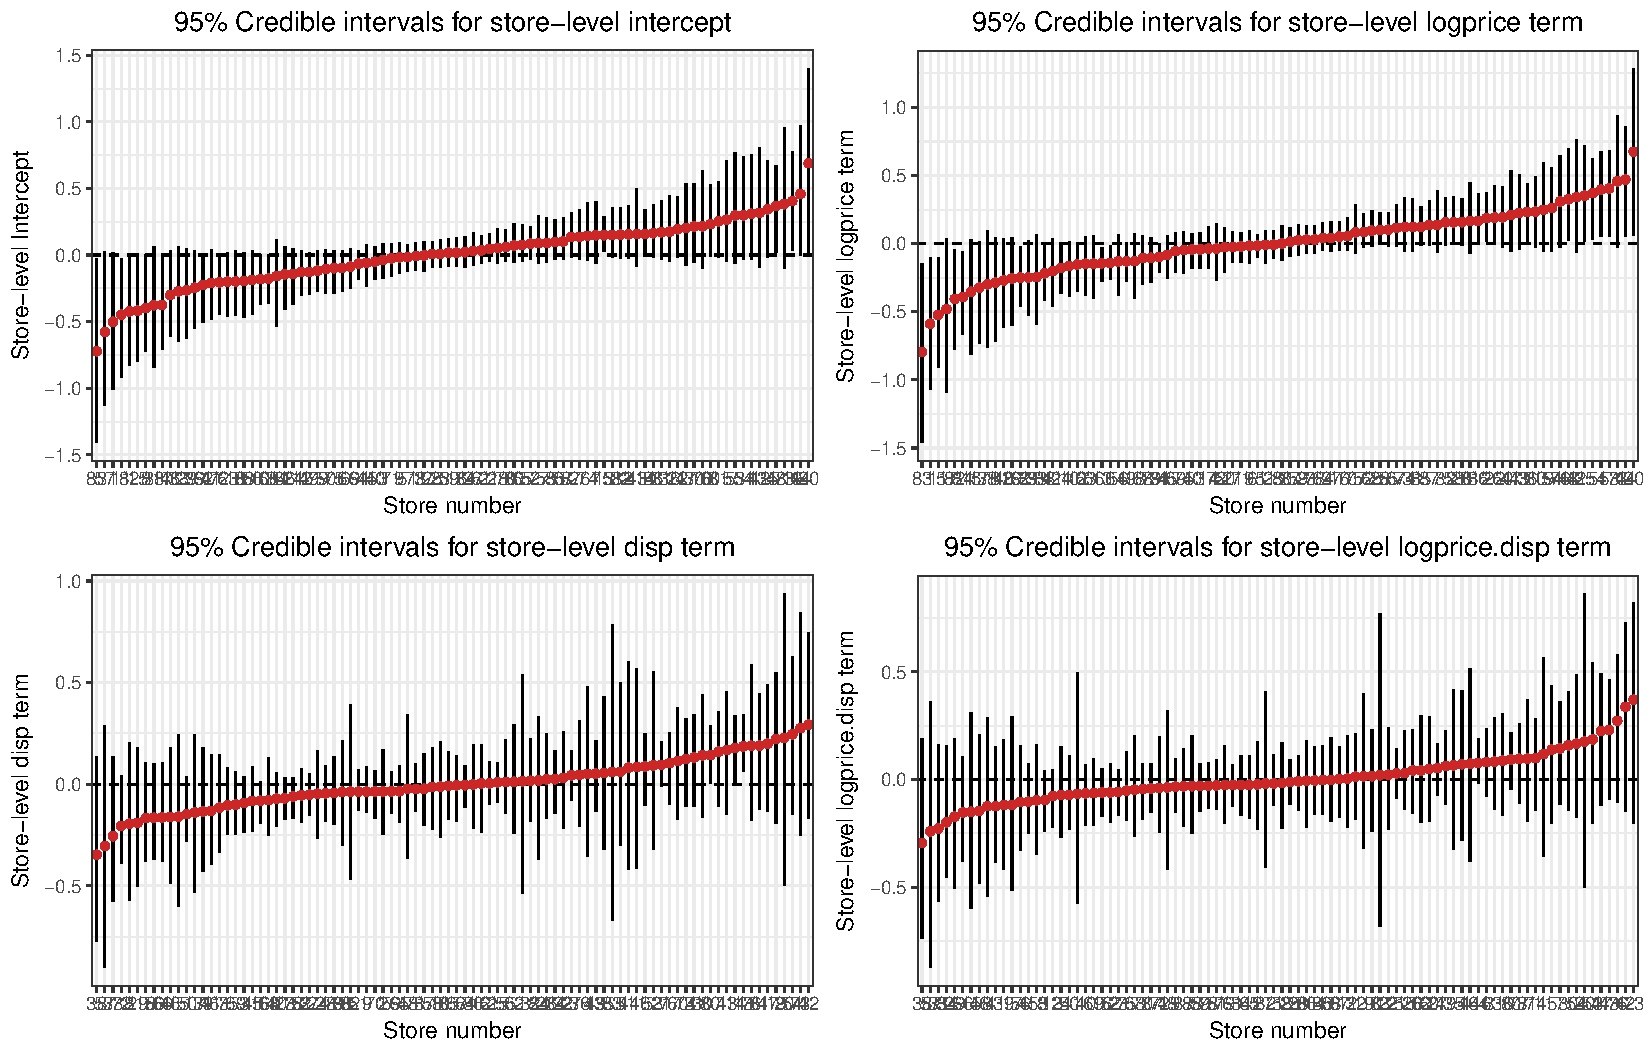
\includegraphics[scale=0.6]{Cheese/img/CIgrid.pdf}
	\caption{Ordered 95\% credible intervals of store-level each store }
	\label{fig:CIgrid}
\end{figure}

\begin{figure}[htp!]
	\centering
		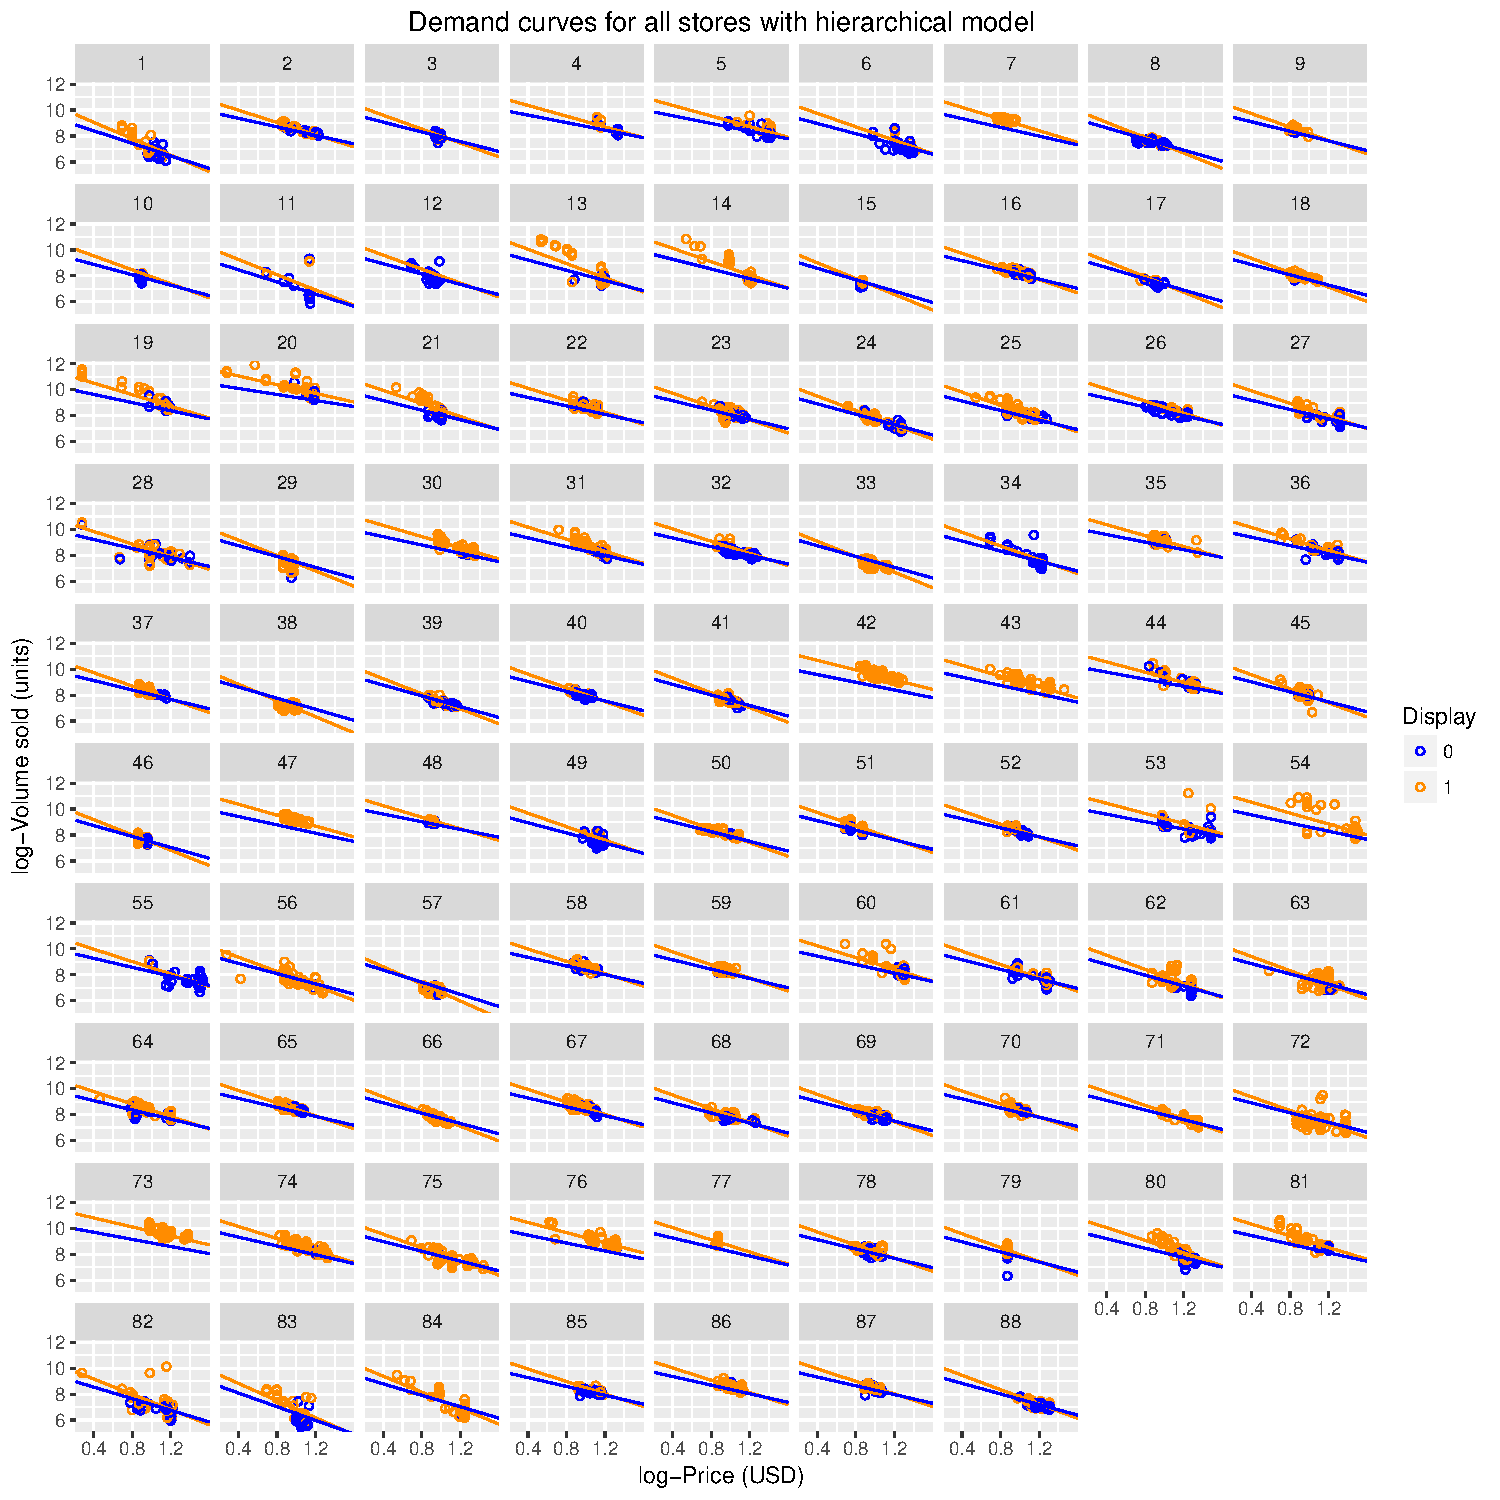
\includegraphics[scale=0.7]{Cheese/img/allfits.pdf}
	\caption{Each store's demand curves with fitted line from Bayesian hierarchical model}
	\label{fig:allfits}
\end{figure}

\end{homeworkProblem}

%----------------------------------------------------------------------------------------
%	PROBLEM 3
%----------------------------------------------------------------------------------------

\pagebreak

\begin{homeworkProblem}

\large
\textbf{A hierarchical probit model via data augmentation}
\normalsize

For this model we model $y_{ij},$  the $j$th binary 0-1 response, $j \in \{ 1, 2, \ldots, n_i \}$, within group $i \in \{ 1, 2, \ldots, I \}$ through the utilization of data augmentation whereby we introduce a latent variable $z_{ij},$
%
%
\begin{align*}
	(z_{ij} | \beta, \gamma_i) &\sim N(x_{ij}^T\beta + w_{ij}^T \gamma_i, 1) \\
	y_{ij} &= \mathbf{1}(z_{ij} > 0) = \begin{cases}
		1 & \text{ if }\; z_{ij} > 0 \\
		0 & \text{ if }\; z_{ij} \leq 0
	\end{cases},
\end{align*}
%
%
where $x_{ij}$ is a vector of covariate features and $w_{ij}$ is a subset of these features whose effects vary at the subject level, captured through $\gamma_i$. We can see that this implies a probit link function so that
%
%
\begin{align*}
	p_{ij} &= P(y_{ij} = 1) = \Phi(x_{ij}^T\beta + w_{ij}^T \gamma_i), 
\end{align*}
%
%
where $\Phi(\cdot)$ is the CDF of the standard normal distribution. Let $z_i$ be the $n_i$-length vector of responses from subject $i,$ and similarly, $X_i$ is a $n_i \times p$ design matrix of subject $i$ and $W_i$ is a $n_i \times q$  design matrix with $q \leq p$ whose columns are a a subset of the columns of $X_i$. We then see that 
%
%
\begin{align*}
	(z_i | \beta, \gamma_i) \sim \pN_{n_i} \left( X_i\beta + W_i \gamma_i , \mathcal{I}_{n_i} \right),
\end{align*}
%
%
and furthermore we model the subject-level responses as coming from a multivatiate normal distribution 
%
%
\begin{align*}
	\gamma_{i} \iid \pN_{q} (0, D),
\end{align*}
%
%
where $D$ is some $q \times q$ covariance matrix. We set the priors for our parameters,
%
%
\begin{align*}
	\pi(\beta) &\propto 1 \\
	\pi(D) &\sim \text{IW}\left( \nu, \Psi \right),
\end{align*}
%
%
and now we can show the full conditionals for the Gibbs sampler. At each iteraton we also need to generate values for the latent variables $z_i$. 
%
%
\begin{align*}
	\pi(\Sigma | \gamma_i) &\sim \text{IW}\left( \nu + I, \Psi + \sum_{i=1}^I \gamma_i \gamma_i^T \right) 
\end{align*}
%
%
\begin{align*}
	\pi\left( \gamma_i | z_i, \beta, D \right) &\propto \pi\left( \gamma_i | D \right) p\left( z_i \right) \\
	&\sim \pN \left( \left[ W_i^T W_i + D^{-1} \right]^{-1} W_i^T (z_i - X_i\beta), \left[ W_i^T W_i + D^{-1} \right]^{-1} \right)
\end{align*}
%
%
\begin{align*}
	\pi(\beta | z, \gamma) &\propto \pi(\beta) \prod_{i=1}^I p\left( z_i | \beta, \gamma_i \right) \\
	&\propto \prod_{i=1}^I \exp\left[ -\frac{1}{2} (z_i - X_i\beta - W_i \gamma_i)^T (z_i - X_i\beta - W_i \gamma_i) \right] \\
	&\sim \pN \left( \left[ \sum_{i=1}^I X_i^T X_i \right]^{-1} \sum_{i=1}^I X_i^T (z_i - W_i\gamma_i), \left[ \sum_{i=1}^I X_i^T X_i \right]^{-1} \right)
\end{align*}
%
%
Finally, the latent variables are generated as follows:
\begin{enumerate}[(1)]
	\item
	\begin{align*}
			\tilde{z}_i \sim \pN_{n_i}(X_i\beta + W_ib_i, I_{n_i})
	\end{align*}
	\item
	For each $z_{ij},$
	\begin{align*}
		z_{ij} | y_{ij} &= \begin{cases}
			\min\{0, \tilde{z}_{ij}\} & \text{if }\; y_{ij} = 1 \\
			\max\{0, \tilde{z}_{ij}\} & \text{if }\; y_{ij} = 0
		\end{cases}
	\end{align*}
\end{enumerate}
%
%
\end{homeworkProblem}


%----------------------------------------------------------------------------------------
%	PROBLEM 4
%----------------------------------------------------------------------------------------

\pagebreak

\begin{homeworkProblem}

\large
\textbf{Gene expression over time}
\normalsize

For this problem, we have measurements of the gene-expression profiles of 14 genes in the \emph{Drosophila} genome tracked over time during embryogenesis. Figure \ref{fig:allgenes} shows the data, faceted by each gene. There are two levels of hierarchy in the data, as demonstrated. Each gene belongs to a cluster, or ``group'' as it is called in this specific context, and each gene has three biological replicates. Figure \ref{fig:bygroups} demonstrates this two-level hierarchical structure; the left column shows the expression profiles for all the genes in each group, and the right column shows the replicates of each gene for a given group. To accomodate the hierarchical and nonlinear time series nature of the data, we introduce a Bayesian hierarchical non-parametric model. \\

Let $i$ be the subscript for clusters of genes, $n$ in the subscript genes, $r$ is the subscript for replicates. If gene $n$ belongs to cluster $i$ we denote this as $n \in c_i,$ and $N_i = \# \left\{ n \in c_i \right\}.$ Each gene $n$ has $N_n$ replicates, and each replicate $r$ of gene $n$ has $N_{nr}$ measuremeants across time. Note that because every array of genes is measured all at once, so each gene has the same $D = \sum_{r=1}^{N_n} N_{nr}$ total measurements across time for all replicates. \\

We can say, for every replicate $r$ of gene $n$, the data we observe take the form of $\y_{nr}$, a $N_{nr} \times 1$ vector observed at times $\tee_{nr}$. Define the following Gaussian processes,
%
%
\begin{align*}
	h_i(t) &\sim \text{GP}(\mathbf{0}, k_h(t, t')) \\
	g_n(t) &\sim \text{GP}(h_i(t), k_g(t, t')) \text{ for } n\in c_i \\
	f_{nr}(t) &\sim \text{GP}(g_n(t), k_f(t, t'))
\end{align*} 
%
%
for some covariance functions $k_h(t, t')$, $k_g(t, t')$, and $k_f(t, t')$. Suppose we have $\h_i$, $\g_n$, and $\f_{nr}$ which is draws from $h_i(t)$, $g_n(t)$, and $f_{nr}(t)$, respectively, at times $\tee_{nr}$. Define $\K_f(\tee_{nr}, \tee_{nr'})$ to be the $N_{nr} \times N_{nr'}$ matrix such that its $(i, j)$ element is $k_g(\tee_{nr}[i], \tee_{nr'}[j])$, and define the matrices $\K_g(\tee_{nr}, \tee_{nr'})$ and $\K_h(\tee_{nr}, \tee_{nr'})$ likewise. Then we model the data $\y_{nr}$ as 
%
%
\begin{align*}
	\y_{nr} &= \f_{nr} + \mathbf{e}, \;\;\mathbf{e} \sim \pN(\mathbf{0}, \sigma^2 \mathcal{I}).
\end{align*}
%
%
We can see the following conditional distributions,
%
%
\begin{align*}
	(\y_{nr} | \f_{nr}) &\sim \pN \left( \f_{nr}, \sigma^2 \mathcal{I} \right) \\
	(\f_{nr} | \g_{n}) &\sim \pN \left( \g_{n}, \K_f(\tee_{nr}, \tee_{nr}) \right) \\
	(\g_{n} | \h_i) &\sim \pN \left( \h_i, \K_g(\tee_{nr}, \tee_{nr}) \right)\\
	(\h_i | \tee_{nr}) &\sim \pN \left( \mathbf{0}, \K_h(\tee_{nr}, \tee_{nr}) \right)
\end{align*}
%
%
It is straightforward to find the marginal likelihood of the data $\y_{nr}$,
%
%
\begin{align*}
	(\y_{nr} | \tee_{nr}, \bm{\uptheta}) \sim \pN \left( \mathbf{0}, \K_h(\tee_{nr}, \tee_{nr}) + \K_g(\tee_{nr}, \tee_{nr}) + \K_f(\tee_{nr}, \tee_{nr})+ \sigma^2 \mathcal{I} \right )
\end{align*}
%
%
where $\bm{\uptheta}$ is a vector which includes the parameters to all of the covariance functions. Now we consider the full data vector for all genes in cluster $i$, $\YY_i = \left\{ \y_n \right\}_{n\in c_i}$ where each $\y_n$ is a concatenation of the replicates in gene $n$, $\y_n = \left\{ \y_{nr} \right\}_{r=1}^{N_n}$, $\tee_n = \left\{ \tee_{nr} \right\}_{r=1}^{N_n} =: \tee$ is the same for each $n$ as illustrated above, and has length $D$, $\mathbf{T}_i = \left\{ \tee_k \right\}_{k \in c_i}$. This will have a marginal full likelihood,
%
%
\begin{align*}
	(\YY_{i} | \mathbf{T}_i, \bm{\uptheta}) &\sim \pN\left( \mathbf{0}, \Sigma_i \right),
\end{align*}
%
%
where $\Sigma_i$ has a matrix which is $N_i \times N_i$ arrangement of block matrices, each of which is of dimension $D \times D$, 
%
%
\begin{align*}
	\Sigma_i[n, n'] &= \begin{cases}
		\K_h(\tee, \tee) + \Sigma_n & \text{if } n = n' \\
		\K_h(\tee, \tee) & \text{otherwise}
	\end{cases},
\end{align*}
%
%
where each $\Sigma_n$ is a covariance matrix representing the with-in gene variance for gene $n$, i.e. the marginal covariance matrix of $\y_n$,
%
%
\begin{align*}
	\Sigma_n[r, r'] &= \begin{cases}
		\K_g(\tee_{nr}, \tee_{nr} ) + \K_f(\tee_{nr}, \tee_{nr} ) + \sigma^2 \mathcal{I}& \text{if } r=r' \\
		\K_g(\tee_{nr}, \tee_{nr'} ) & \text{otherwise}
	\end{cases}
\end{align*}
%
%
and also notice that each block $\Sigma_n[r, r']$ is of dimension $N_{nr} \times N_{nr'}$. \\

%
Now suppose we want to find the conditional distribution of ``new'' draws from the Gaussian grocesses given the data we observe. Specifically we want to find the distribution of $\h_i^\star$ drawn at $\tee^\star_i$, $\g_n^\star$ at $\tee^\star_n$, and $\f_{nr}^\star$ at $\tee^\star_{nr}$, conditional on the data. First, it is easy to find the respective marginal distributions of each of these,
%
%
\begin{align*}
	(\h_i^\star | \tee_i^\star) &\sim \pN \left( \mathbf{0}, \K_h(\tee_i^\star, \tee_i^\star) \right) \\
	(\g_n^\star | \tee_n^\star) &\sim \pN \left( \mathbf{0}, \K_h(\tee_n^\star, \tee_n^\star ) + \K_g(\tee_n^\star, \tee_n^\star) \right) \\
	(\f_{nr}^\star | \tee_{nr}^\star) &\sim \pN \left( \mathbf{0}, \K_h(\tee_{nr}^\star, \tee_{nr}^\star ) + \K_g(\tee_{nr}^\star, \tee_{nr}^\star) + \K_f(\tee_{nr}^\star, \tee_{nr}^\star) \right).
\end{align*}
%
%
Conditioned on $\y_i$, the distribution of each becomes 
%
%
\begin{align*}
	\begin{bmatrix}
		\YY_i \\
		\h_i^\star
	\end{bmatrix} &\sim \pN \left( 0, \begin{bmatrix}
		\Sigma_i & \K_{i\star}^T \\
		\K_{i\star} & \K_{i \star \star}
	\end{bmatrix} \right) \\
	%
	\begin{bmatrix}
		\YY_i \\
		\g_n^\star
	\end{bmatrix} &\sim \pN \left( 0, \begin{bmatrix}
		\Sigma_i & \K_{n\star}^T \\
		\K_{n\star} & \K_{n \star \star}
	\end{bmatrix} \right) \\
	%
	\begin{bmatrix}
		\YY_i \\
		\f_{nr}^\star
	\end{bmatrix} &\sim \pN \left( 0, \begin{bmatrix}
		\Sigma_i & \K_{nr\star}^T \\
		\K_{nr\star} & \K_{nr \star \star}
	\end{bmatrix} \right),
\end{align*}
%
%
where
%
%
\begin{align*}
	\K_{i \star \star} &= \K_h(\tee_i^\star, \tee_i^\star)\\
	\K_{n \star \star} &= \K_h(\tee_n^\star, \tee_n^\star ) + \K_g(\tee_n^\star, \tee_n^\star) \\ 
	\K_{nr \star \star} &= \K_h(\tee_{nr}^\star, \tee_{nr}^\star ) + \K_g(\tee_{nr}^\star, \tee_{nr}^\star) + \K_f(\tee_{nr}^\star, \tee_{nr}^\star)
\end{align*}
%
%
and the elements of the off-diagonal matrices are given as
%
%
\begin{align*}
	\K_{i\star}[t, t'] &= \text{cov}\left( \h_i^\star[t], \YY_i[t'] \right) = k_h(t, t') \\
	%
	\K_{n \star}[t, t'] &= \text{cov} \left( \g_n^\star[t], \YY_i[t'] \in \y_{n} \right) = \begin{cases}
		k_h(t, t') + k_g(t, t') & \text{if } n = n' \\
		k_h(t, t') & \text{otherwise} 
	\end{cases} \\
	%
	\K_{nr \star}[t, t'] &= \text{cov} \left( \f_{nr}^\star[t], \YY_i[t'] \in \y_{n'r'} \right) = \begin{cases}
		k_h(t, t') + k_g(t, t') + k_f(t, t') & \text{if } n = n' \text{ and } r=r' \\
		k_h(t, t') + k_g(t, t') & \text{if } n = n' \text{ and } r\neq r' \\
		k_h(t, t') & \text{otherwise}. 
	\end{cases}
\end{align*}
%
With all this in hand, the conditional distributions may be written explicitly, e.g.
%
%
\begin{align*}
	(\h_i^\star | \YY_i) &\sim \pN \left( \K_{i\star}\Sigma_i^{-1} \YY_i, \K_{i\star\star} - \K_{i\star}\Sigma_{i}^{-1}\K_{i\star}^T \right).
\end{align*}
%
%
The challenge now is to choose the hyperparameters within $\mathbf{\uptheta}$ by maximizing the marginal likelihood of the full data vector, $\YY_i$. In my \textsf{R} script, I used the \texttt{optim} command to do this, which by default uses the Nelder-Mead method of optimization. For this application, we use the squared-exponential with zero ``nugget'' parameter, e.g., for the cluster-level Gaussian process,
%
%
\begin{align*}
	k_h(t, t') &= \alpha_h \cdot \exp\left[ -\frac{(t - t')^2}{\gamma_h} \right].
\end{align*}

Results of the HGP regression are shown below, at the group, gene, and replicate level for all three groups. The estimated time series functions are shown, along with a 95\% confidence band. Not that we have strange results for Group 1. The estimated optimal $\gamma_h$ parameter obtained by \texttt{optim} for Group 1 is very high, around $e^{13}$ This is likely due to a very flat likelihood function, due to the fact that the data all look very similar to each other. The high value of $\gamma_h$ gives a matrix $\K_h(\mathbf{t}, \mathbf{t})$ which has very large numbers in most of its elements, which may have been a source of numerical instability in \textsf{R}.

 % Exploiting the fact that each $\y_n$ has the same $\tee_n = \tee$ and therefore the same $\Sigma_n$, and defining $\K_h = \K_h(\tee, \tee)$ as a shorthand and $\bar{\y}_i = \sum_{k\in c_i} \y_k / N_i$, \href{Hensmen et al. (2013)}{https://bmcbioinformatics.biomedcentral.com/articles/10.1186/1471-2105-14-252} showed that the log-marginal likelihood can be expressed as
%
%
% \begin{align*}
% 	\log p(\YY_i | \mathbf{\uptheta}) =& C + \frac{1}{2} \log \left| \K_h \right| + \frac{N_i}{2}\log \left| \Sigma_n \right| + \frac{1}{2} \log \left| \K_h^{-1} + N_i \Sigma_n \right| - \ldots \\
% 	& \frac{1}{2} \left[ \sum_{k \in c_i} \y_k^T \Sigma_n^{-1} \y_k - N_i^2 \bar{\y}_i^T \Sigma_n^{-1} \left( \K_h^{-1} + \Sigma_n^{-1} \right)^{-1} \Sigma_n^{-1} \bar{\y}_i \right],
% \end{align*}
%
%
% where $C$ is a constant. This takes $\mathcal{O}(D^3)$ time to compute instead of $\mathcal{O}(N_i^3 D^3)$ time as would take if we did not use this property. In this case we can use a black-box optimizer such as the Nelder-Mead method in order to find these optimal parameters. \\

% https://bmcbioinformatics.biomedcentral.com/articles/10.1186/1471-2105-14-252

\begin{figure}[htp!]
	\centering
		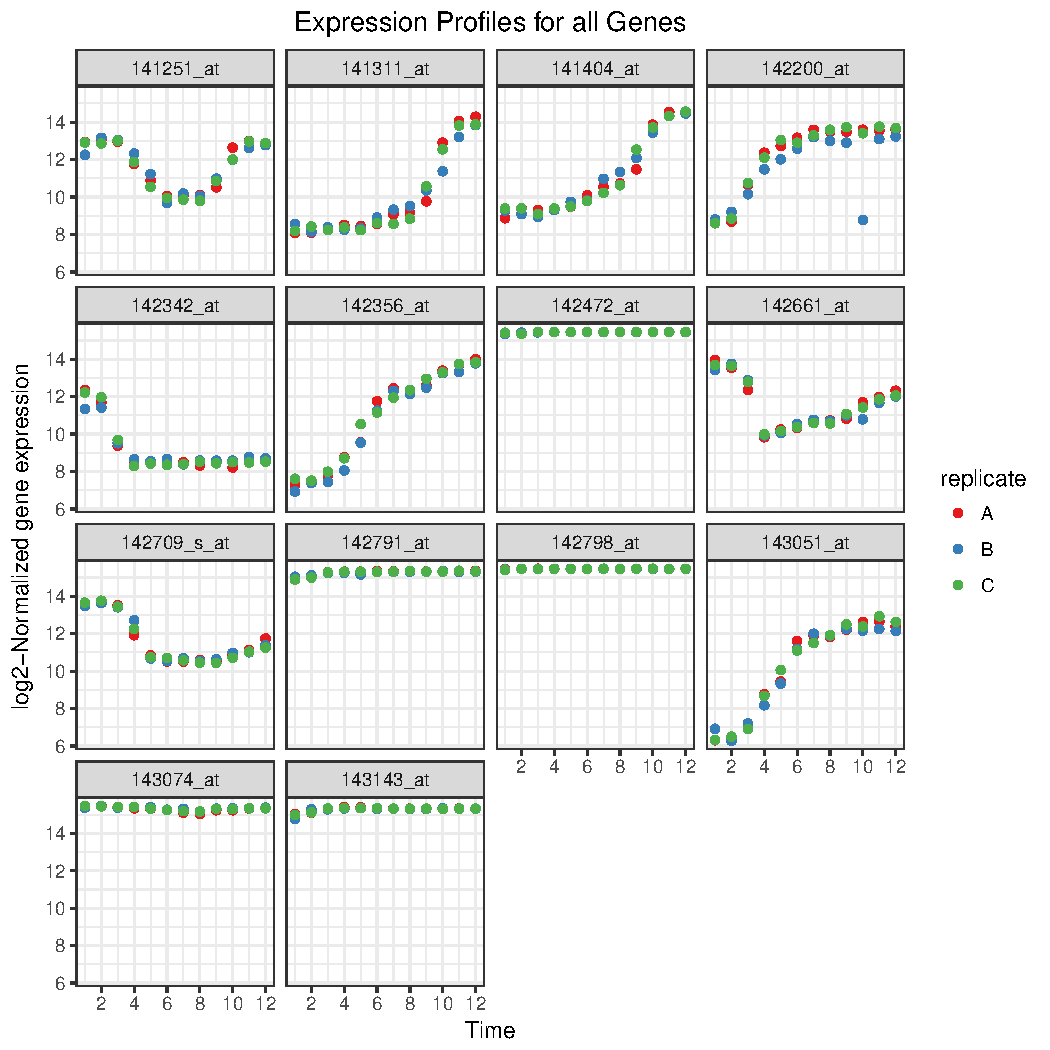
\includegraphics[scale=0.8]{Drosophila/img/allgenes.pdf}
	\caption{Expression profiles for each gene across all replicates}
	\label{fig:allgenes}
\end{figure}

\begin{figure}[htp!]
	\centering
		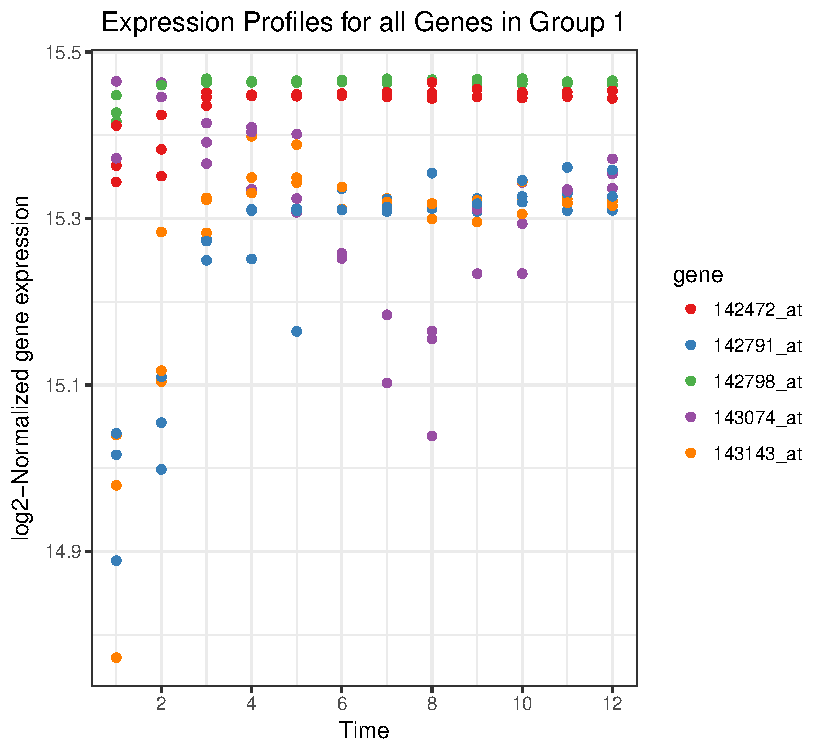
\includegraphics[scale=0.5]{Drosophila/img/allgenes1.pdf} 
		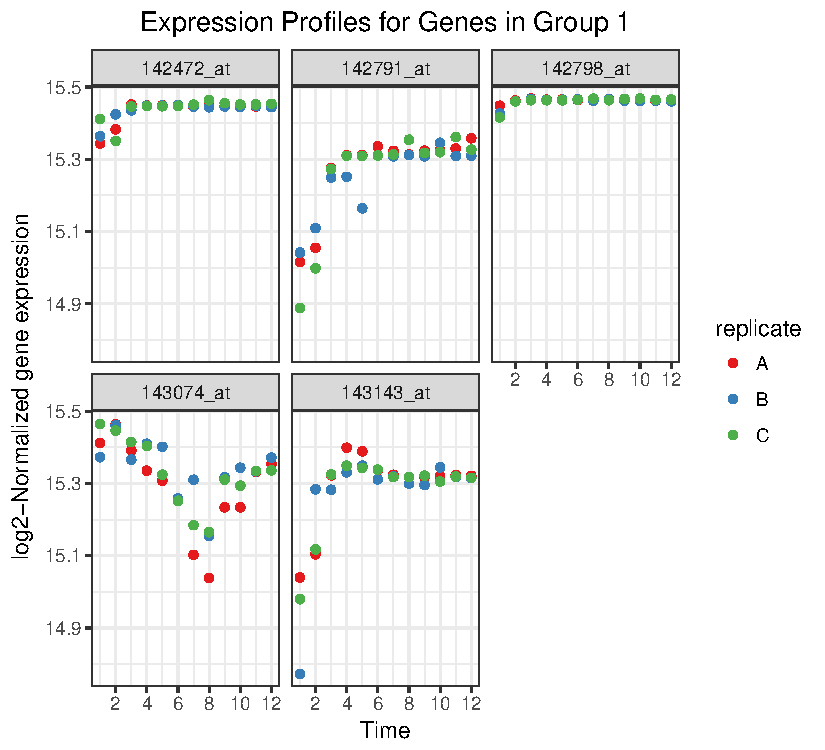
\includegraphics[scale=0.5]{Drosophila/img/facetgroup1.pdf} \\
		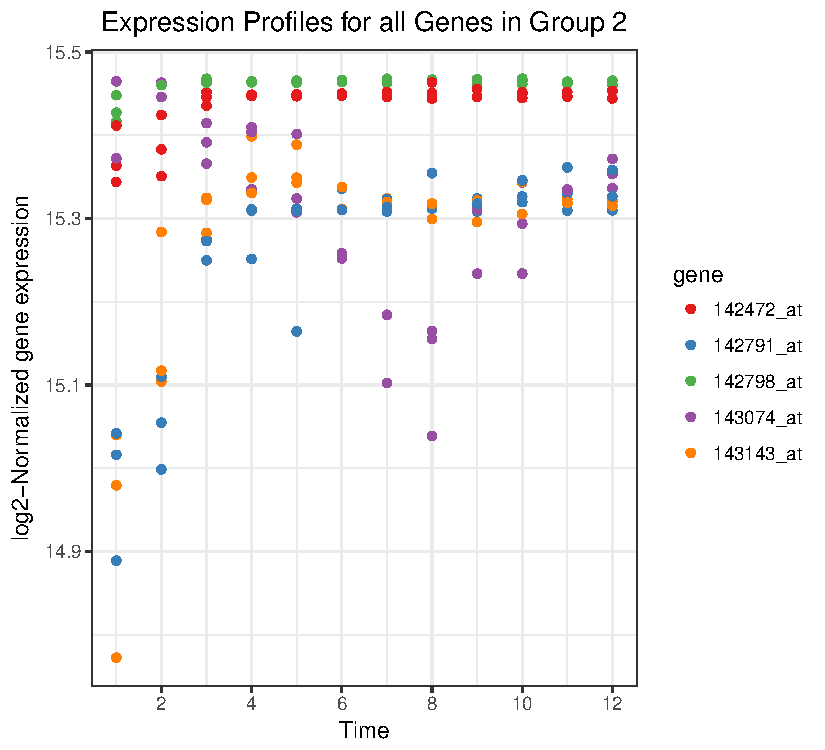
\includegraphics[scale=0.5]{Drosophila/img/allgenes2.pdf} 
		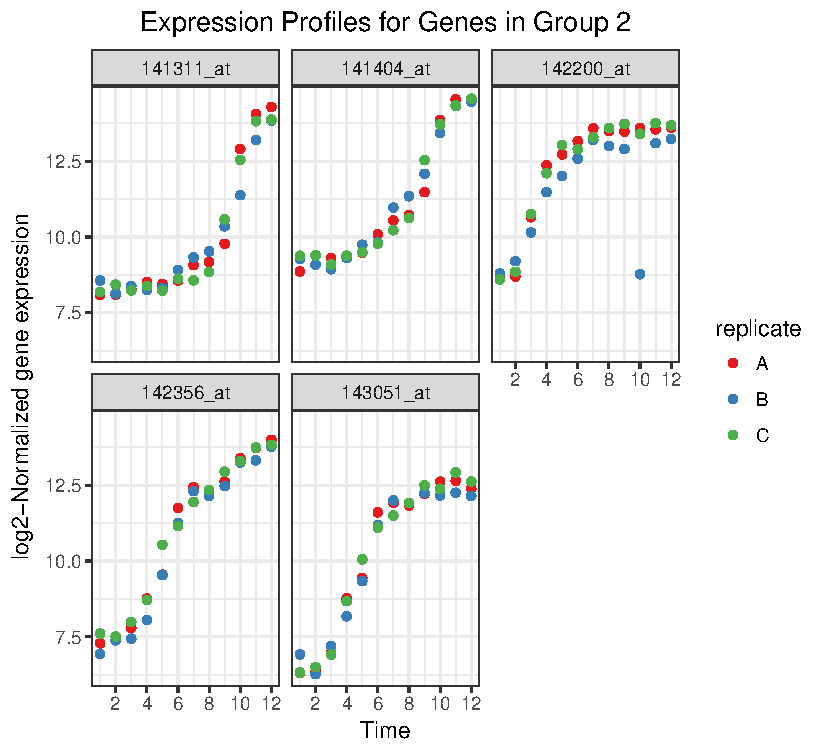
\includegraphics[scale=0.5]{Drosophila/img/facetgroup2.pdf} \\
		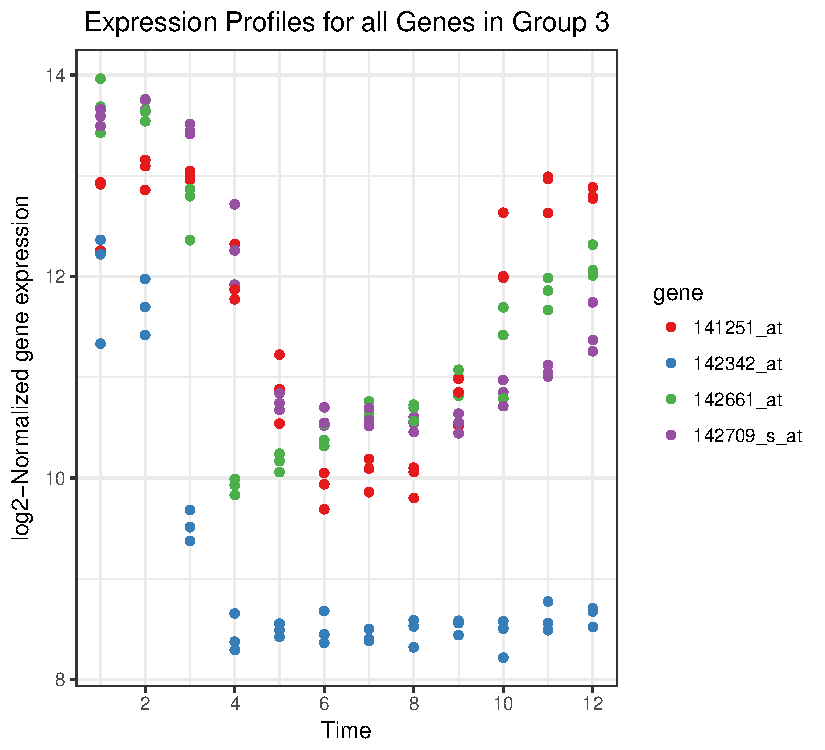
\includegraphics[scale=0.5]{Drosophila/img/allgenes3.pdf} 	
		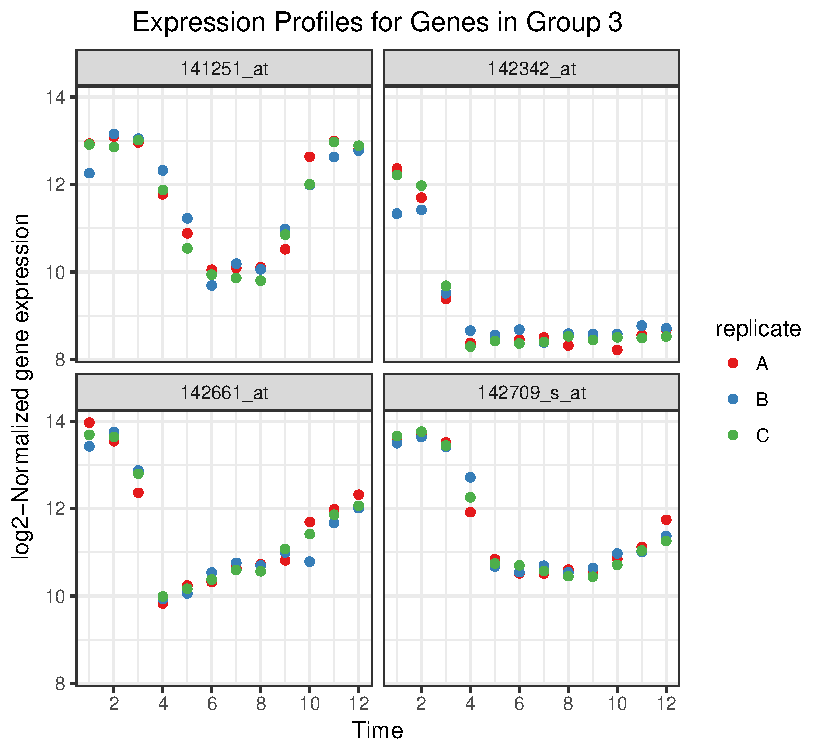
\includegraphics[scale=0.5]{Drosophila/img/facetgroup3.pdf}
	\caption{Expression profiles of all genes, accounting for clusters (or ``groups'') and replicates}
	\label{fig:bygroups}
\end{figure}

%%%%% 
%%%%% GROUP 1
%%%%% 

\pagebreak

\begin{figure}[htp!]
	\centering
		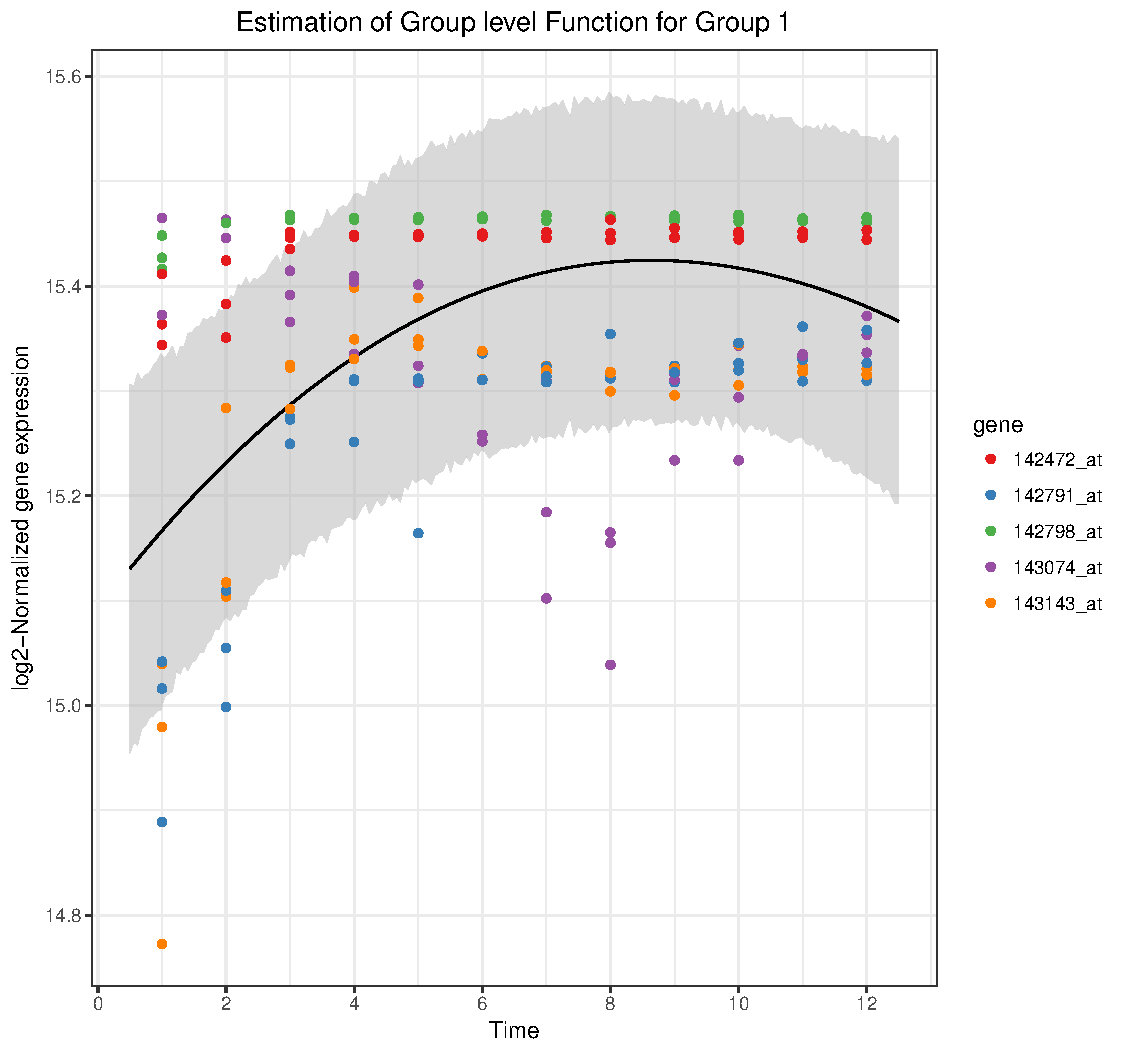
\includegraphics[scale=0.6]{Drosophila/img/GPgroup1_group.pdf} \\
		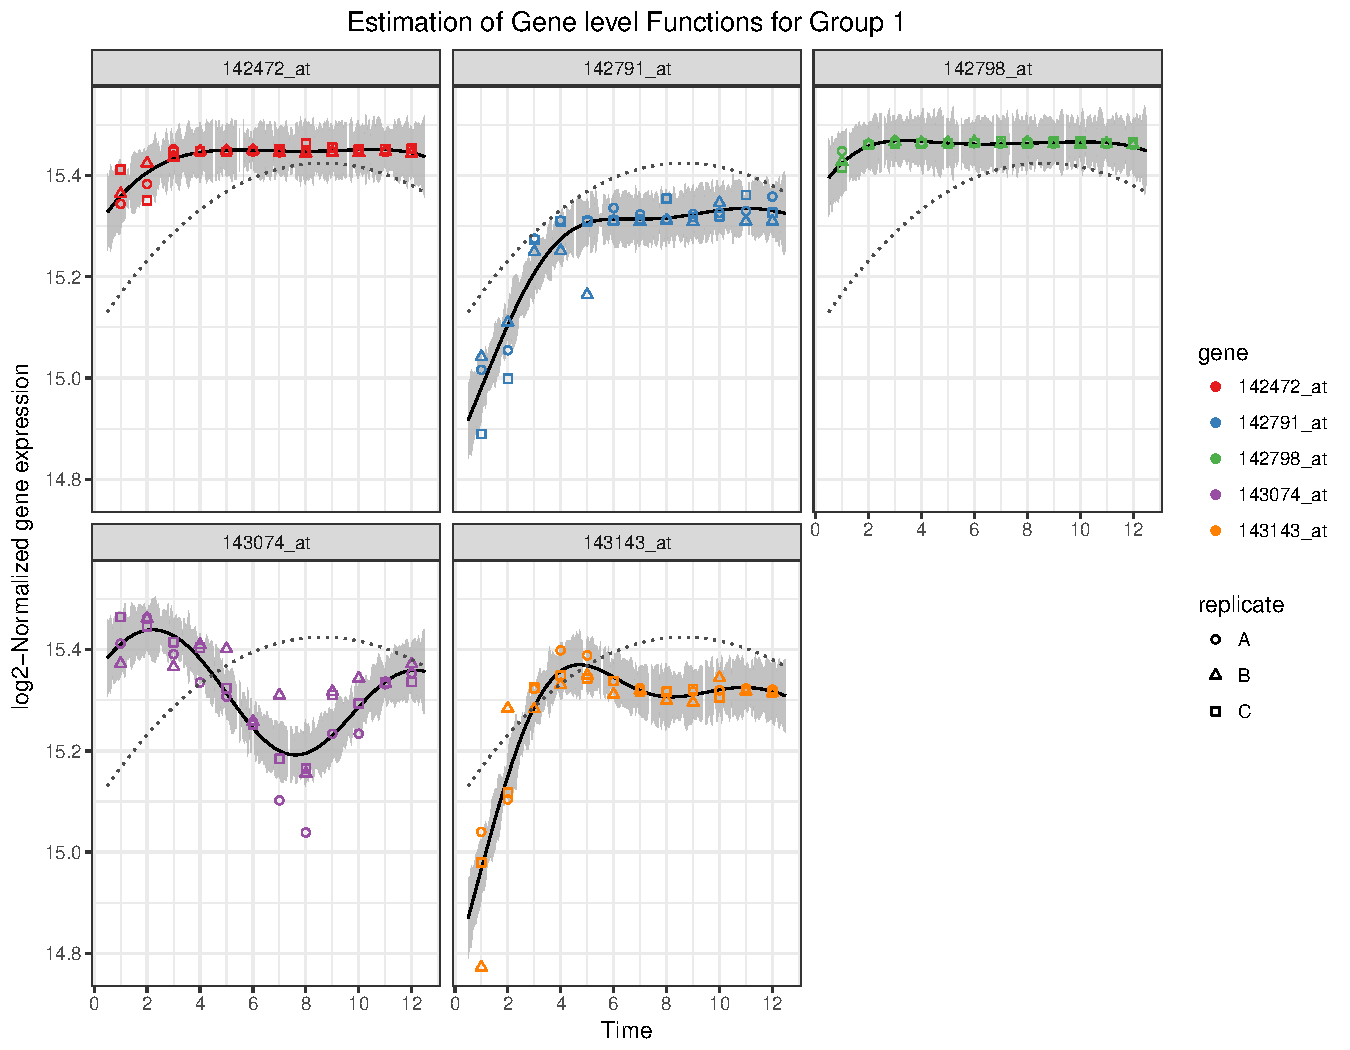
\includegraphics[scale=0.6]{Drosophila/img/GPgroup1_genes.pdf} 
	\caption{Estimation of group- and gene-level gene expression time series functions for Group 1}
	\label{fig:GPgroup1}
\end{figure}


\pagebreak

\begin{figure}[htp!]
	\centering
		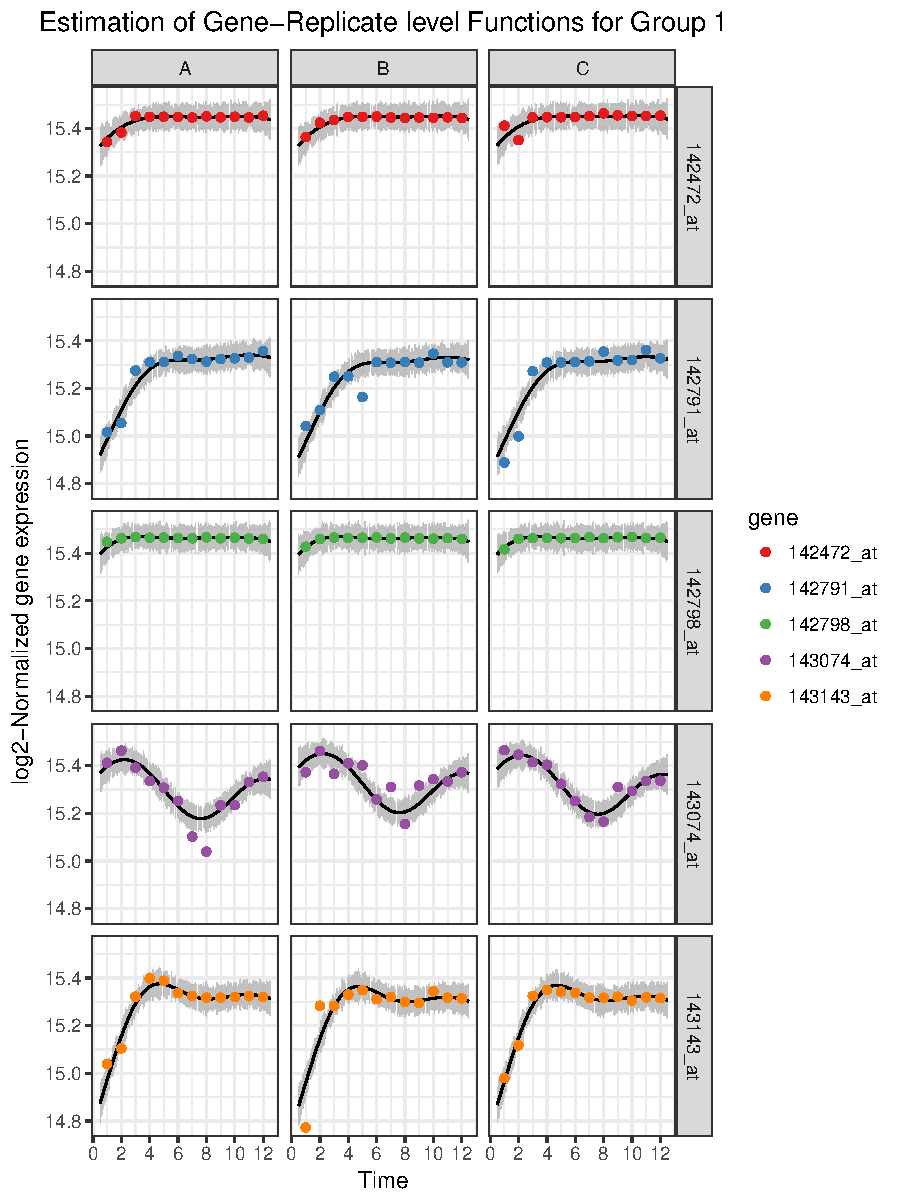
\includegraphics[scale=1]{Drosophila/img/GPgroup1_replicates.pdf}
	\caption{Estimation of gene, replicate-level gene expression time series functions for genes in Group 1}
	\label{fig:reps1}
\end{figure}


%%%%% 
%%%%% GROUP 2
%%%%% 

\pagebreak

\begin{figure}[htp!]
	\centering
		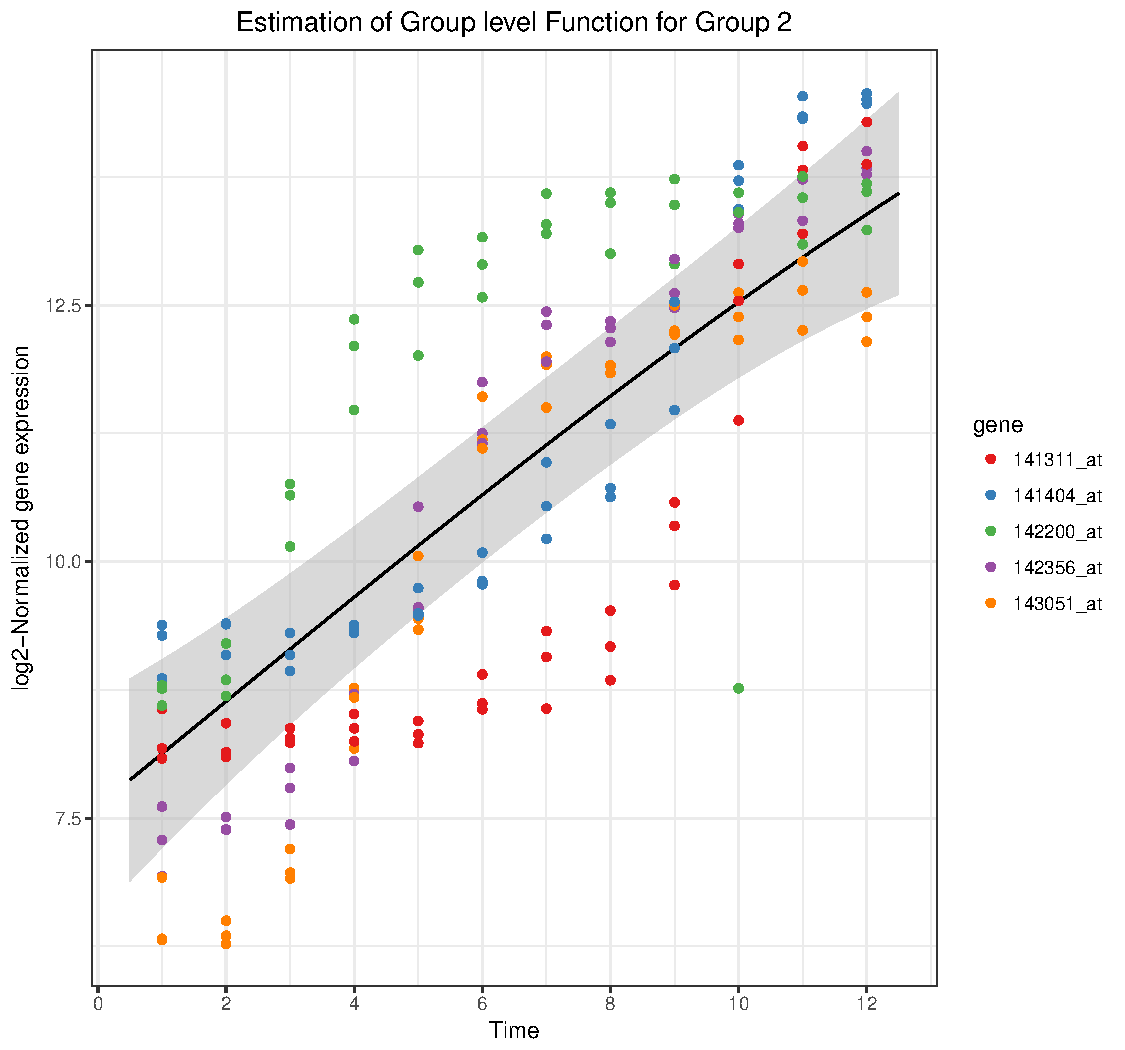
\includegraphics[scale=0.6]{Drosophila/img/GPgroup2_group.pdf} \\
		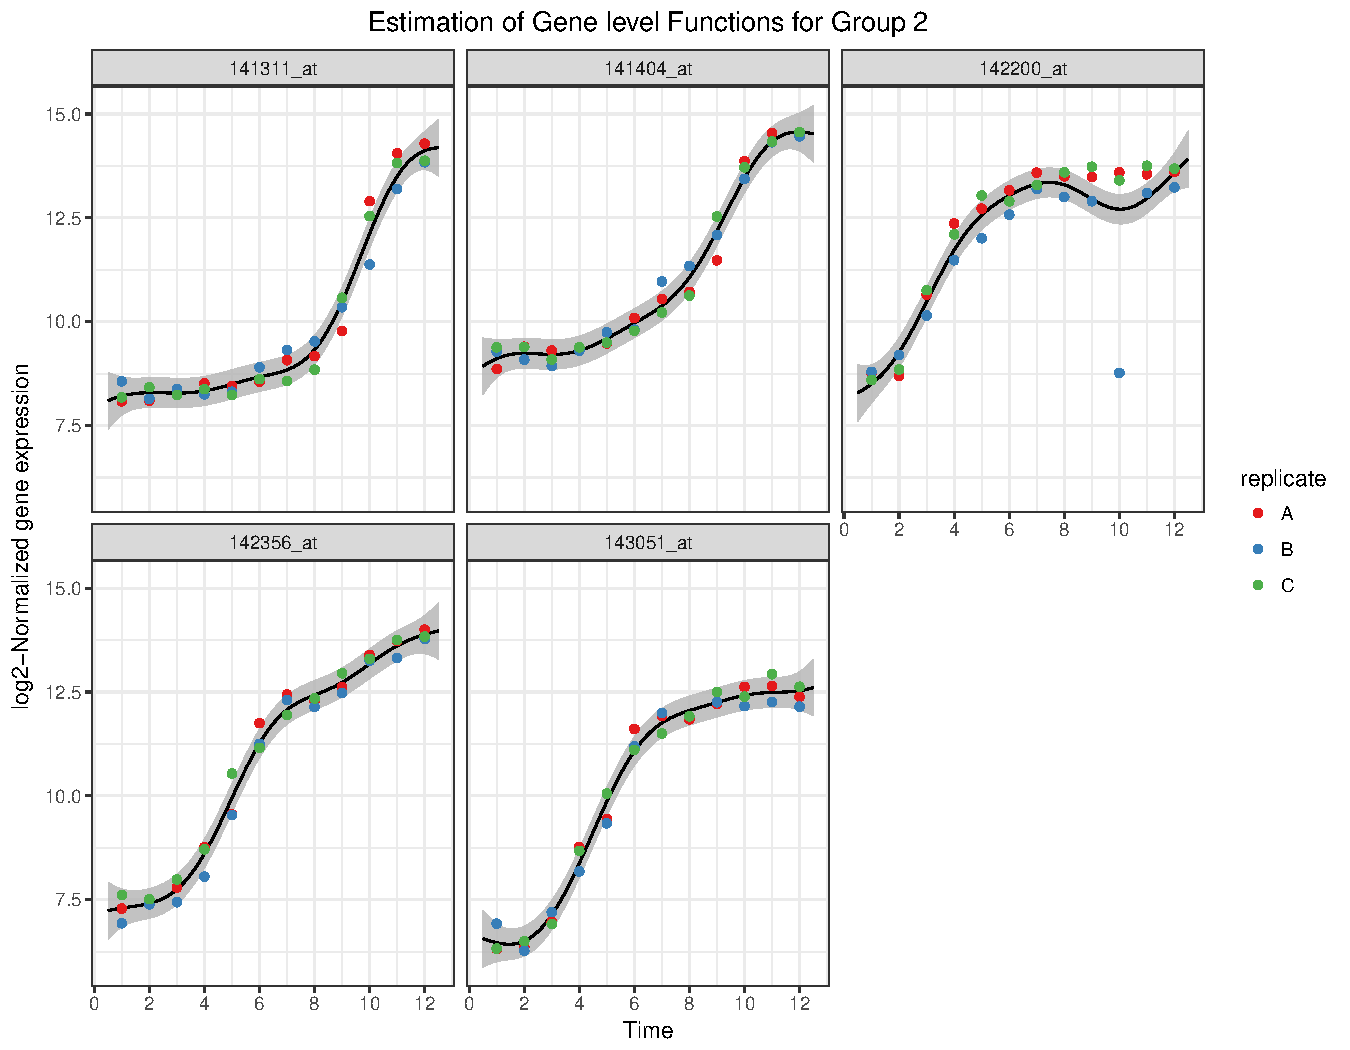
\includegraphics[scale=0.6]{Drosophila/img/GPgroup2_genes.pdf} 
	\caption{Estimation of group- and gene-level gene expression time series functions for Group 2}
	\label{fig:GPgroup2}
\end{figure}

\pagebreak

\begin{figure}[htp!]
	\centering
		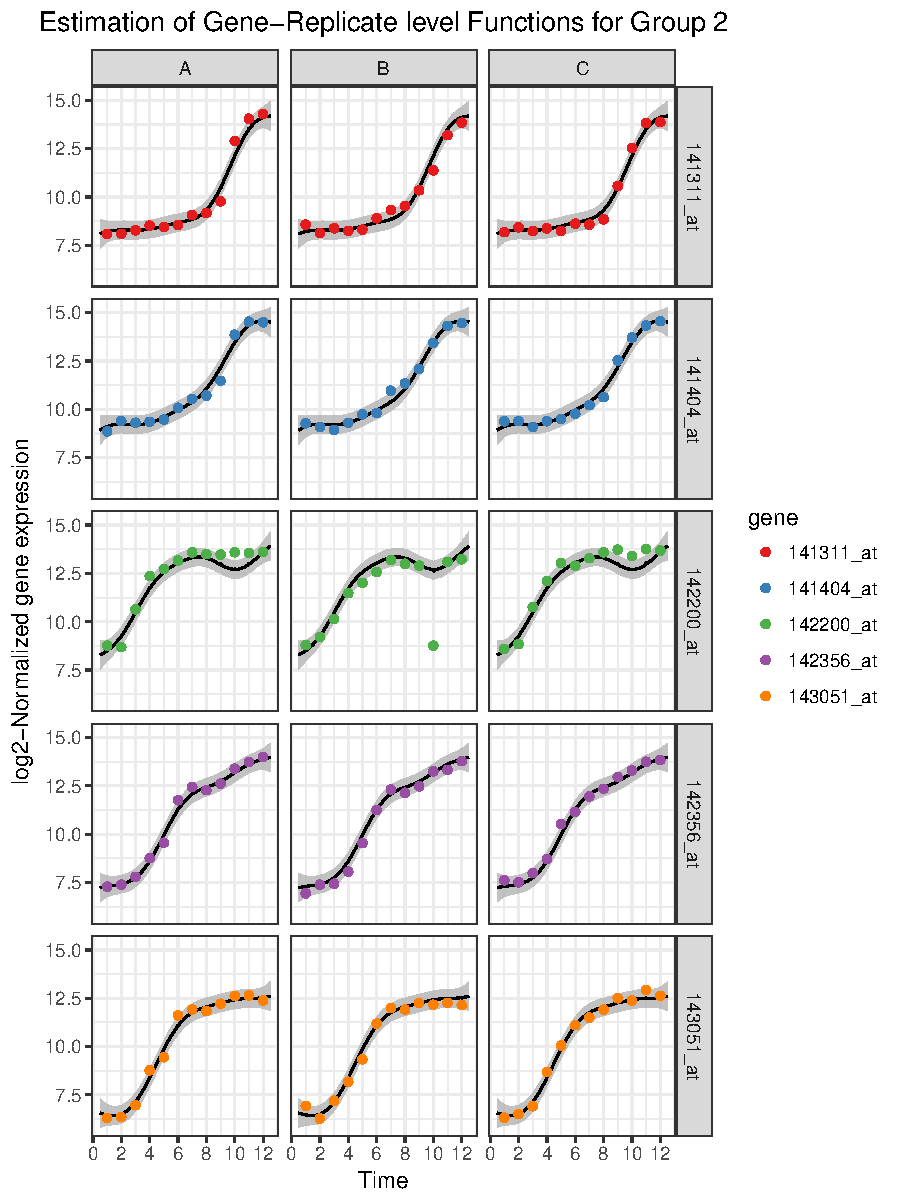
\includegraphics[scale=1]{Drosophila/img/GPgroup2_replicates.pdf}
	\caption{Estimation of gene, replicate-level gene expression time series functions for genes in Group 2}
	\label{fig:reps2}
\end{figure}

\pagebreak

%%%%% 
%%%%% GROUP 3
%%%%% 

\pagebreak

\begin{figure}[htp!]
	\centering
		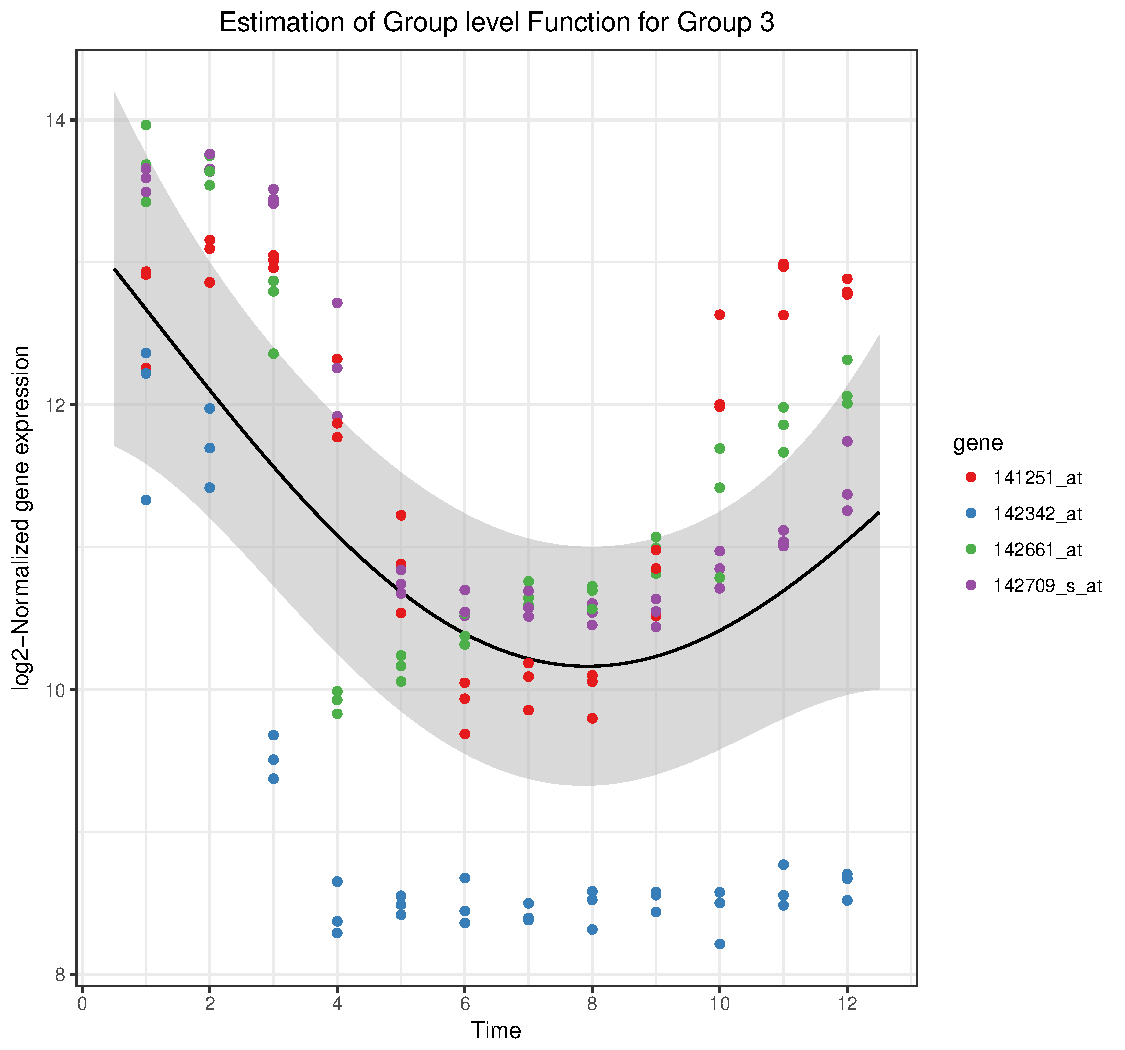
\includegraphics[scale=0.6]{Drosophila/img/GPgroup3_group.pdf} \\
		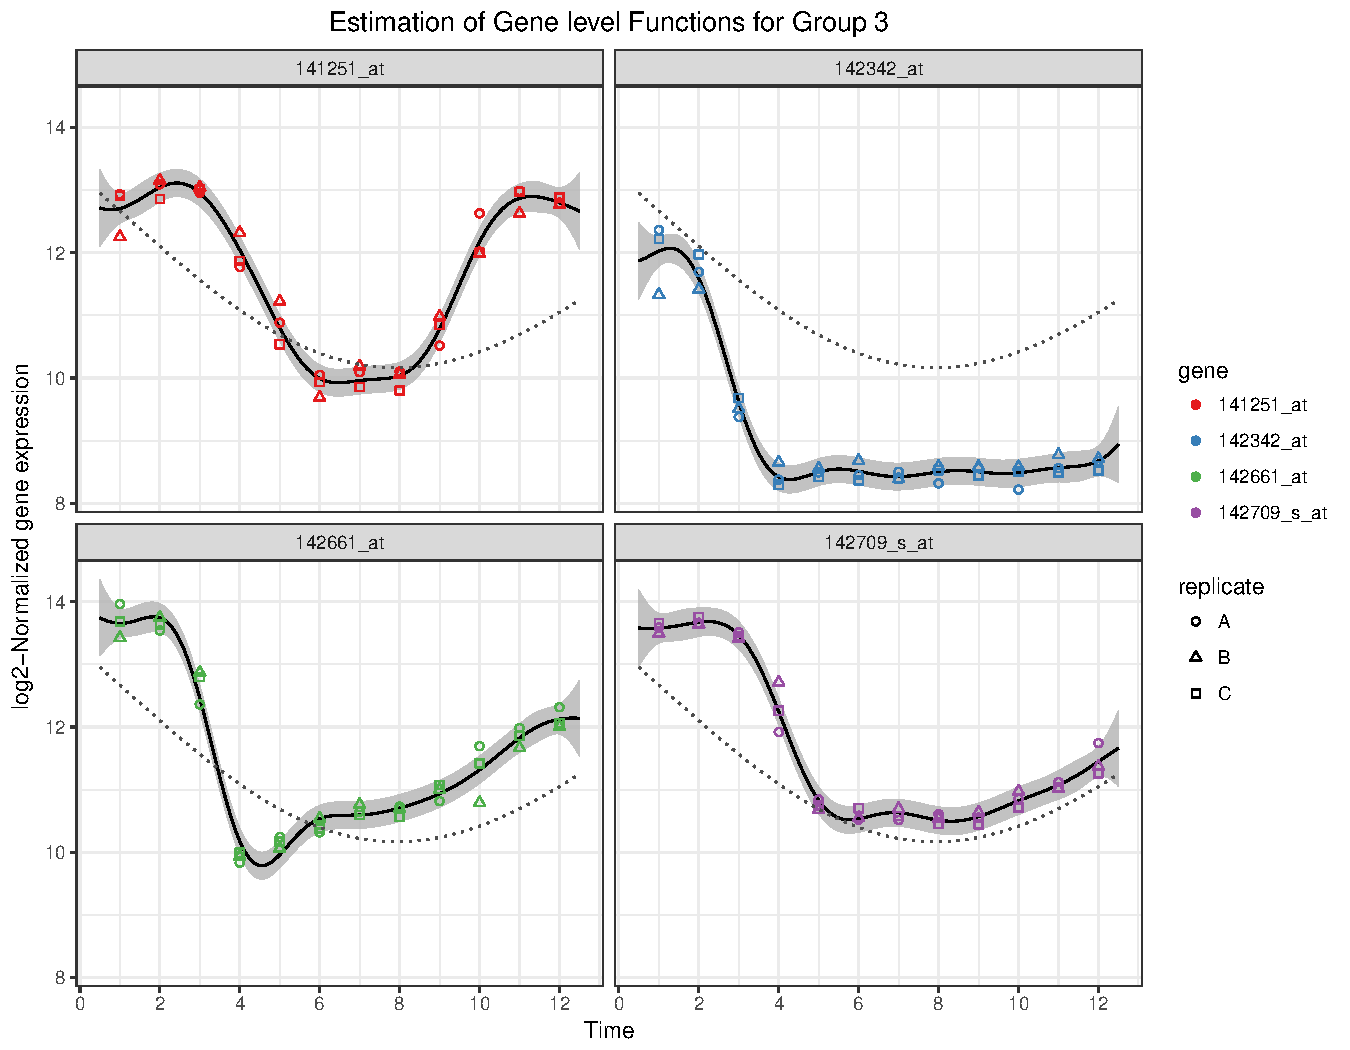
\includegraphics[scale=0.6]{Drosophila/img/GPgroup3_genes.pdf} 
	\caption{Estimation of group- and gene-level gene expression time series functions for Group 3}
	\label{fig:GPgroup3}
\end{figure}


\begin{figure}[htp!]
	\centering
		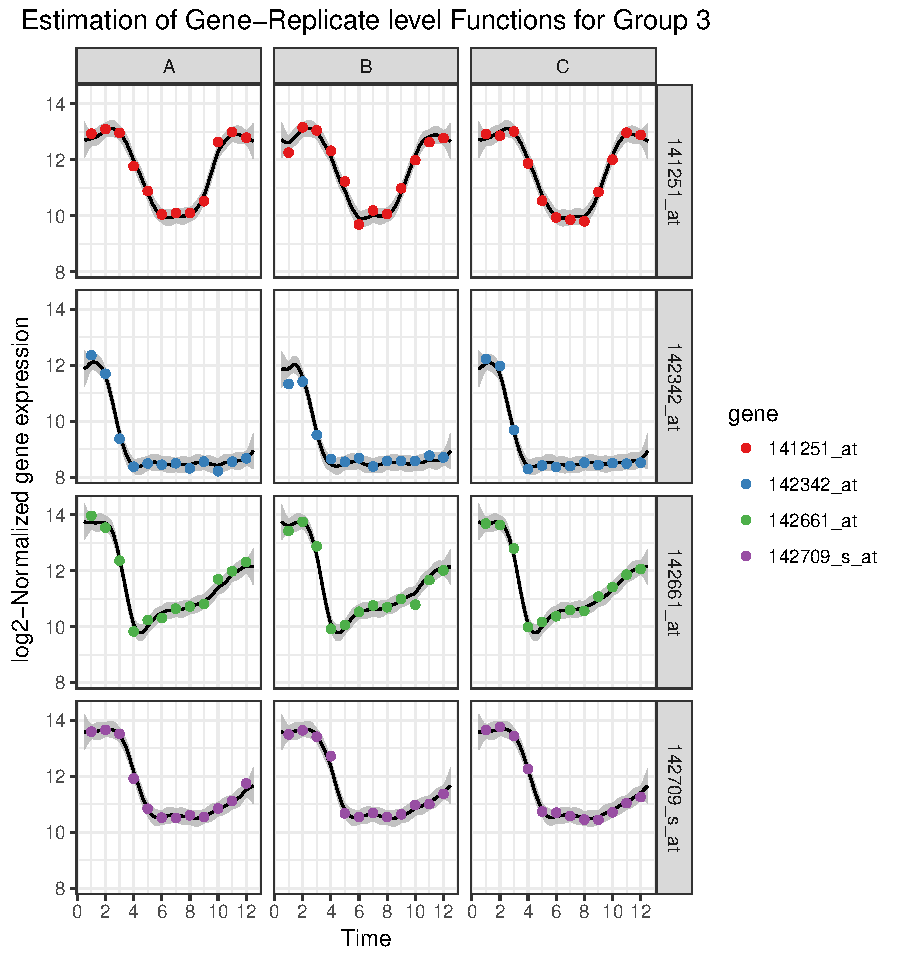
\includegraphics[scale=1]{Drosophila/img/GPgroup3_replicates.pdf}
	\caption{Estimation of gene, replicate-level gene expression time series functions for genes in Group 3}
	\label{fig:reps3}
\end{figure}

%
%
\end{homeworkProblem}


%%----------------------------------------------------------------------------------------
%%	LIST CODE
%%----------------------------------------------------------------------------------------
%
% \pagebreak
% % \rscript{homework03.r}{Sample Perl Script With Highlighting}
% R code for \texttt{myfuns03.R}
% \lstinputlisting[language=R]{myfuns03.R}
% \pagebreak
% R code for \texttt{exercises03.R}
% \lstinputlisting[language=R]{exercises03.R}
%

%----------------------------------------------------------------------------------------

\end{document}